% Options for packages loaded elsewhere
\PassOptionsToPackage{unicode}{hyperref}
\PassOptionsToPackage{hyphens}{url}
\documentclass[
]{article}
\usepackage{xcolor}
\usepackage{amsmath,amssymb}
\setcounter{secnumdepth}{-\maxdimen} % remove section numbering
\usepackage{iftex}
\ifPDFTeX
  \usepackage[T1]{fontenc}
  \usepackage[utf8]{inputenc}
  \usepackage{textcomp} % provide euro and other symbols
\else % if luatex or xetex
  \usepackage{unicode-math} % this also loads fontspec
  \defaultfontfeatures{Scale=MatchLowercase}
  \defaultfontfeatures[\rmfamily]{Ligatures=TeX,Scale=1}
\fi
\usepackage{lmodern}
\ifPDFTeX\else
  % xetex/luatex font selection
\fi
% Use upquote if available, for straight quotes in verbatim environments
\IfFileExists{upquote.sty}{\usepackage{upquote}}{}
\IfFileExists{microtype.sty}{% use microtype if available
  \usepackage[]{microtype}
  \UseMicrotypeSet[protrusion]{basicmath} % disable protrusion for tt fonts
}{}
\makeatletter
\@ifundefined{KOMAClassName}{% if non-KOMA class
  \IfFileExists{parskip.sty}{%
    \usepackage{parskip}
  }{% else
    \setlength{\parindent}{0pt}
    \setlength{\parskip}{6pt plus 2pt minus 1pt}}
}{% if KOMA class
  \KOMAoptions{parskip=half}}
\makeatother
\usepackage{longtable,booktabs,array}
\newcounter{none} % for unnumbered tables
\usepackage{calc} % for calculating minipage widths
% Correct order of tables after \paragraph or \subparagraph
\usepackage{etoolbox}
\makeatletter
\patchcmd\longtable{\par}{\if@noskipsec\mbox{}\fi\par}{}{}
\makeatother
% Allow footnotes in longtable head/foot
\IfFileExists{footnotehyper.sty}{\usepackage{footnotehyper}}{\usepackage{footnote}}
\makesavenoteenv{longtable}
\usepackage{graphicx}
\makeatletter
\newsavebox\pandoc@box
\newcommand*\pandocbounded[1]{% scales image to fit in text height/width
  \sbox\pandoc@box{#1}%
  \Gscale@div\@tempa{\textheight}{\dimexpr\ht\pandoc@box+\dp\pandoc@box\relax}%
  \Gscale@div\@tempb{\linewidth}{\wd\pandoc@box}%
  \ifdim\@tempb\p@<\@tempa\p@\let\@tempa\@tempb\fi% select the smaller of both
  \ifdim\@tempa\p@<\p@\scalebox{\@tempa}{\usebox\pandoc@box}%
  \else\usebox{\pandoc@box}%
  \fi%
}
% Set default figure placement to htbp
\def\fps@figure{htbp}
\makeatother
\setlength{\emergencystretch}{3em} % prevent overfull lines
\providecommand{\tightlist}{%
  \setlength{\itemsep}{0pt}\setlength{\parskip}{0pt}}
\usepackage{bookmark}
\IfFileExists{xurl.sty}{\usepackage{xurl}}{} % add URL line breaks if available
\urlstyle{same}
\hypersetup{
  hidelinks,
  pdfcreator={LaTeX via pandoc}}

\author{}
\date{}

\begin{document}

Design description of

Wisdom Computing Persperctive


\includegraphics[width=5.75764in,height=2.5375in,alt={}]{./media_en/media/image1.png}

{\def\LTcaptype{none} % do not increment counter
\begin{longtable}[]{@{}
  >{\centering\arraybackslash}p{(\linewidth - 2\tabcolsep) * \real{0.2143}}
  >{\centering\arraybackslash}p{(\linewidth - 2\tabcolsep) * \real{0.7786}}@{}}
\toprule\noalign{}
\endhead
\bottomrule\noalign{}
\endlastfoot
Author： & TianYi Yu \\
Name： & rainbow\_yu \\
GitHub： & \url{https://github.com/rainbowyuyu} \\
\end{longtable}
}

April 2025

\section{catalogue}\label{catalogue}

\hyperref[section]{abstract 5}

\hyperref[foreword]{1 Introduction 6}

\hyperref[motive]{1.1 Motivation 6}

\hyperref[the-problem-to-be-solved]{1.2 Problems to be solved 6}

\hyperref[work-on-this-paper]{1.3 Work of this paper 7}

\hyperref[related-work]{2 Related work 7}

\hyperref[hand-written-numeral-recognition]{2.1 Handwritten number
recognition 7}

\hyperref[corner-detection-algorithm]{2.2 Corner detection algorithm 8}

\hyperref[yolo-neural-network]{2.3YOLO neural network 8}

\hyperref[mamba-backbone-network]{2.4 Mamba backbone network 8}

\hyperref[data-collection-and-annotation]{3 Data collection and
annotation 8}

\hyperref[the-raw-data-set]{3.1 Original data set 8}

\hyperref[data-set-generation]{3.2 Data set generation 9}

\hyperref[key-methods]{Four key methods 14}

\hyperref[mathematical-equation-detection]{4.1 Mathematical formula
detection 14}

\hyperref[mathematical-equation-model-training]{4.1.1 Mathematical
formula model training 14}

\hyperref[formula-image-preprocessing]{4.1.2 Formula image preprocessing
16}

\hyperref[formula-content-detection]{4.1.3 Formula content detection 18}

\hyperref[mathematical-formula-number-extraction]{4.1.4 Extraction of
numbers from mathematical expressions 19}

\hyperref[step-by-step-solution-animation-module]{4.2 Step-by-step
solution animation module 20}

\hyperref[step-by-step-solution-frame-by-frame-rendering-method]{4.2.1
Step-by-step solution frame by frame rendering method 21}

\hyperref[the-control-scheme-for-each-animation-element]{4.2.2 Control
scheme for each animation element 21}

\hyperref[build-basic-formula-animation-class]{4.2.3 Build basic
calculation animation class 22}

\hyperref[monocular-operation-is-divided-into-step-by-step-animation-construction]{4.2.4
Single operation step-by-step calculation animation construction 23}

\hyperref[two-eye-operation-is-divided-into-step-by-step-animation-construction]{4.2.5
Dual vision operation step-by-step animation construction 25}

\hyperref[experiment]{5 Experiments 27}

\hyperref[data]{5.1 Data 27}

\hyperref[benchmark-model]{5.2 Benchmark model 27}

\hyperref[appraisal-procedure]{5.3 Evaluation method 29}

\hyperref[mean-average-accuracy]{5.3.1 Mean accuracy mean 29}

\hyperref[accuracy]{5.3.2 accuracy 29}

\hyperref[recall]{5.3.3 recall 29}

\hyperref[f1-value]{5.3.4 F1 value 29}

\hyperref[experimental-configuration]{5.4 Experimental configuration 30}

\hyperref[experimental-platform]{5.4.1 Experimental platform 30}

\hyperref[hyperparameter-settings]{5.4.2, Hyperparameter Settings 30}

\hyperref[training-process]{5.4.3 Training process 30}

\hyperref[experimental-result]{5.5 Experimental results 30}

\hyperref[analysis-and-discussion]{6 Analysis and discussion 32}

\hyperref[interface-for-interaction]{7 Interaction interface 33}

\hyperref[mathematical-formula-input-interface]{7.1 Mathematical formula
input interface 33}

\hyperref[mathematical-formula-calculation-interface]{7.2 Mathematical
formula calculation interface 34}

\hyperref[free-input-board-interface]{7.3 Free input drawing board
interface 35}

\hyperref[sum-up]{8. Summary 36}

\hyperref[sum-up-1]{8.1 Summary 36}

\hyperref[look-into-the-distance]{8.2 Outlook 37}

\hyperref[reference-documentation]{reference documentation 37}

\section{}\label{section}

\section{abstract}\label{abstract}

this graduation design aims to develop and research a handwriting matrix
recognition and step-by-step visual calculation process display system,
addressing the issue of abstract formulas and complex calculation steps
that students find difficult to understand when learning mathematics. By
integrating artificial intelligence with visualization animation
technology, the system enhances precise recognition of handwritten
matrix content through the introduction of Mamba backbone networks,
completes digital extraction and matrix reconstruction using the YOLO
model, and simultaneously combines CoordAttention coordinate attention
mechanisms to improve the accurate grasp of character spatial positions.
The calculation process is demonstrated frame by frame through the Manim
animation engine, vividly showcasing each mathematical calculation step,
helping students intuitively understand the intrinsic logic of
mathematical operations. Through dynamically generating animation
processes for different computational tasks, the system exhibits high
modularity and flexibility, capable of generating various mathematical
operation examples in real-time according to student needs. By
innovating human-computer interaction methods, it brings mathematical
calculation processes to life, helping students bridge the gap between
knowledge and understanding on a deeper level, ultimately achieving a
learning experience where "every step is understood." The
system\textquotesingle s scalability and interactivity make it an
intuitive, user-friendly, and efficient auxiliary tool in education.

\section{foreword}\label{foreword}

\subsection{motive}\label{motive}

In today\textquotesingle s higher education system, which increasingly
emphasizes competency and practical application, students not only need
to accumulate knowledge but also face the challenge of understanding and
applying this knowledge. This is especially true in mathematics courses,
where many students are often bogged down by complex formulas and
computational steps, unable to truly grasp the underlying reasoning.
Particularly in linear algebra and matrix computation courses, students
lack an intuitive understanding of formulas and frequently make mistakes
during calculations, failing to effectively build a systematic knowledge
framework. This issue is particularly prominent in the current
educational environment, especially in advanced courses, where
students\textquotesingle{} understanding remains superficial, lacking
deep reflection and practice. With the development of information
technology, there are tools available on the market such as Microsoft
Math and MathDF that provide some computational support, but these tools
mostly focus on providing final results, neglecting students
\textquotesingle need for a detailed understanding of the calculation
process. More importantly, these tools lack personalization and
interactivity, failing to offer customized support based on different
students\textquotesingle{} learning progress and comprehension levels.

\subsection{The problem to be solved}\label{the-problem-to-be-solved}

Data Set Generation In the field of mathematics learning and
computation, especially in the teaching of matrix operations, existing
datasets mostly focus on areas such as image recognition and text
classification, with relatively few dedicated to mathematical matrix
recognition. This presents certain challenges when constructing training
sets. Particularly for handwritten matrix recognition, the lack of
datasets results in insufficient coverage of different writing styles
and matrix sizes.

The accuracy of image recognition: Existing object detection algorithms,
such as YOLO (You Only Look Once) and {[}1{]}, have been widely applied
to tasks like object detection and image classification, demonstrating
excellent performance in real-time processing and accuracy. However,
image recognition of handwritten matrices faces numerous challenges,
including font variations, noise interference, and image blurriness, all
of which can affect the precision of recognition.

Mathematical Expression Localization After completing the recognition of
matrix images, the next major challenge is to accurately locate the
identified elements in relation to the positions of mathematical
expressions. Different matrix calculations involve various mathematical
operators, such as addition, multiplication, and determinants. The
positions and functions of these symbols in mathematical expressions
need to be accurately identified and positioned.

The extensibility of the code framework is crucial as technology
continues to evolve and requirements change. During the system design
phase, adopting a modular development approach ensures minimal
dependencies between functional modules, making it easier to modify and
upgrade these modules later on. This also facilitates rapid updates and
real-time collaboration for front-end and back-end interfaces, as well
as the expansion of functionalities.

\subsection{Work on this paper}\label{work-on-this-paper}

To address the aforementioned issues, this project integrates artificial
intelligence and visual animation technology to propose an innovative
human-computer interaction method. The system, by incorporating
YOLO-Mamba{[}2{]} image recognition technology and the Manim animation
engine, can accurately identify handwritten matrices uploaded by
students and present the entire computational process through dynamic
animations. Unlike traditional mathematics teaching tools, this system
not only focuses on displaying the results but also emphasizes the
process, using clear visual derivations to help students understand the
logic and principles behind each computational step.

Image Recognition: This project employs the YOLO-Mamba object detection
algorithm, which, through an optimized training dataset, enhances the
accuracy of recognizing handwritten matrices. The YOLO algorithm, by
learning from multi-layer convolutional neural networks, can effectively
identify each element in the matrix, overcoming issues such as
variations in handwriting, noise interference, and image blurriness,
ensuring high-precision recognition results.

The automated generation of animation processes allows the system to
dynamically create corresponding computational process animations based
on the matrix size, type, and required mathematical operations input by
users, without human intervention. This mechanism is built on the
modular sub-components and unified data interfaces of the Manim
animation engine, enabling the system to achieve high flexibility and
scalability. Whether it\textquotesingle s matrix operations of different
scales or various row-column determinants, addition, multiplication, and
other operations, the system can automatically generate the
corresponding animation effects, significantly enhancing user experience
and interactivity.

Maintainability and Scalability To ensure the maintainability and
scalability of the system, this project adopted a modular development
approach, ensuring the independence and extensibility of each functional
module. Through unified data interfaces and templated structures, the
system can easily expand new mathematical operation functions and
quickly update and maintain them in later stages. In particular, the
design of the system ensures that new features can be rapidly deployed
and supports multi-tasking and multi-scenario applications, enabling the
system to meet evolving educational needs. All work in this document has
been uploaded to https://github.com/rainbowyuyu/animate\_cal, and all
tasks can be reproduced according to the README instructions, with
requests available for expansion and maintenance. The visualization
platform address is
\url{https://wisdom-computing-perspective.streamlit.app/}, and the front
end is updated in real-time through accessing the GitHub stream.

\section{related work}\label{related-work}

\subsection{hand-written numeral
recognition}\label{hand-written-numeral-recognition}

Handwritten digit recognition technology has made significant progress,
especially in the development of deep learning, where methods based on
Convolutional Neural Networks (CNNs) {[}3{]} have gradually become
mainstream. CNNs can efficiently extract features from images through
multiple layers of convolution and pooling operations, which is
particularly advantageous when dealing with diverse characters and
complex backgrounds, compared to traditional Optical Character
Recognition (OCR) {[}4{]} methods such as edge detection, color
analysis, and template matching. Although they have achieved good
results on standard datasets, they often require longer training times
and computational resources. Therefore, adopting more efficient CNN
architectures, especially for handling noisy and complex background
handwritten digits, remains a direction worth exploring.

\subsection{Corner detection
algorithm}\label{corner-detection-algorithm}

Corner detection is a key task in computer vision, widely applied in
image matching, motion tracking, and other fields. The Harris corner
detection algorithm {[}5{]} evaluates the gray level changes of local
windows through a self-correlation matrix to determine whether corners
exist in the image. The Shi-Tomasi algorithm {[}6{]}, an improvement
over the Harris algorithm, uses local brightness gradient information
and structural matrix eigenvalues for corner detection, which better
resists noise and enhances robustness. Despite its stronger
adaptability, it has higher computational complexity and requires
large-scale labeled data for training.

\subsection{YOLO neural network}\label{yolo-neural-network}

YOLO algorithm is a real-time object detection method based on
Convolutional Neural Networks (CNN). The core innovation of YOLO lies in
transforming the object detection task into a regression problem,
directly outputting the class of the object and its bounding box
coordinates through a single forward pass of the entire image. Unlike
traditional object detection methods, YOLO can effectively capture small
objects in images with low spatial resolution and reduce the likelihood
of background misidentification. However, for tasks like handwritten
equations that require capturing details and contextual information from
the image, as well as adding attention recognition, improvements are
still needed.

\subsection{Mamba backbone network}\label{mamba-backbone-network}

Mamba backbone network is a convolutional neural network architecture
proposed in recent years for visual tasks, aiming to improve the
performance of traditional convolutional networks in complex visual
tasks. Compared with other backbone networks, Mamba network introduces
dynamic convolution and adaptive feature fusion mechanisms, enabling it
to more effectively capture image details and contextual information.

\section{Data collection and
annotation}\label{data-collection-and-annotation}

\subsection{The raw data set}\label{the-raw-data-set}

The original data set "Handwritten math symbols dataset" has 82 classes,
including their own operation symbols and numbers and letters. Each
class contains about 10,000 black and white images in jpg format of
45x45. The url of the data set is
https://www.kaggle.com/datasets/xainano/handwrittenmathsymbols/data.

\begin{figure}
\centering
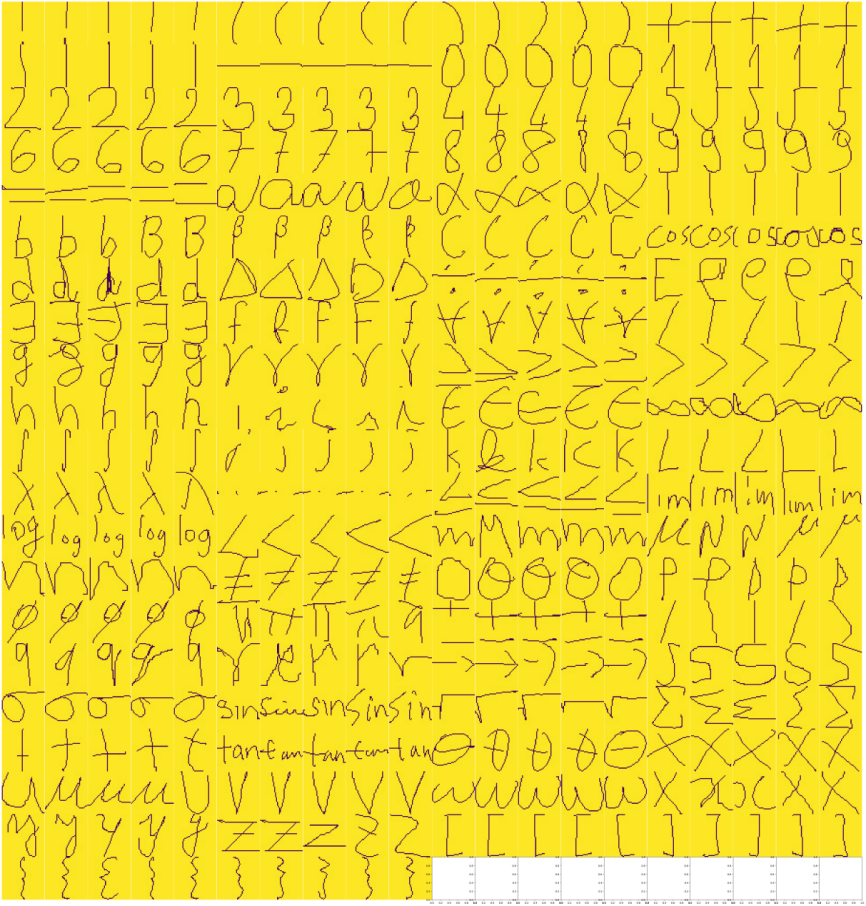
\includegraphics[width=3.93701in,height=4.11707in,alt={,  }]{./media_en/media/image2.png}
\caption{Figure 3.1 Sample of the original data set}
\end{figure}

\subsection{Data set generation}\label{data-set-generation}

The data set generation adopts the operations of adding alpha channel,
image transverse and longitudinal transformation, adding noise and so on
in digital image processing. Multiple versions of iterations and
attempts are carried out, and finally the automatic data set generation
and automatic annotation functions are realized.

The version iteration of the data set generator is also an important
basis for the model version iteration. The basis for the version
performance iteration when the model is introduced later is the version
of the data set.

The automatic generation and annotation of data sets solve the huge
workload of manual writing data sets and labelimg annotation.

\begin{longtable}[]{@{}
  >{\centering\arraybackslash}p{(\linewidth - 2\tabcolsep) * \real{0.4784}}
  >{\centering\arraybackslash}p{(\linewidth - 2\tabcolsep) * \real{0.4784}}@{}}
\caption{Table 3.1 Summary of data set versions}\tabularnewline
\toprule\noalign{}
\endfirsthead
\endhead
\bottomrule\noalign{}
\endlastfoot
\textbf{edition} & \textbf{function} \\
v0 & Randomly arrange the numbers \\
v1 & Add an alpha channel \\
v2 & Generate matrix elements \\
v3 & generated matrix \\
v4 & Generate a stable handwritten matrix \\
\end{longtable}

\begin{enumerate}
\def\labelenumi{\arabic{enumi}.}
\item
  v0
\end{enumerate}

\begin{quote}
Read all files and build a list, randomly select an element and place it
in a random position of random size. When generating annotations, change
the width and height of the annotations with random values.

Problems caused by v0: The upper layer elements cover the lower layer,
and the image in the label is not complete, resulting in very serious
overfitting.
\end{quote}

{\def\LTcaptype{none} % do not increment counter
\begin{longtable}[]{@{}
  >{\centering\arraybackslash}p{(\linewidth - 2\tabcolsep) * \real{0.5000}}
  >{\centering\arraybackslash}p{(\linewidth - 2\tabcolsep) * \real{0.5000}}@{}}
\toprule\noalign{}
\endhead
\bottomrule\noalign{}
\endlastfoot
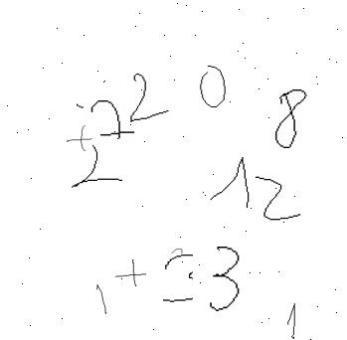
\includegraphics[width=1.575in,height=1.54375in,alt={image\_50004}]{./media_en/media/image3.jpeg}

Figure 3.2 Sample images generated by v0 &
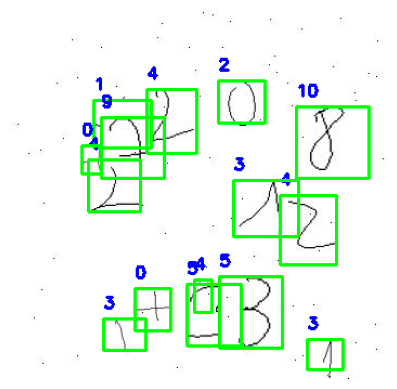
\includegraphics[width=1.575in,height=1.54306in,alt={,  }]{./media_en/media/image4.png}

Figure 3.3 Sample annotated by v0 \\
\end{longtable}
}

\begin{quote}
Note: The labels in the image are the categories of the image, and their
classes mapping relationship is: {[}\{0: +\}, \{1: -\}, \{2: 0\}, \{3:
1\}, \{4: 2\}, \{5: 3\}, \{6: 4\}, \{7: 5\}, \{8: 6\}, \{9: 7\},
\{10:8\}, \{11:9\}, \{12: =\}, \{13: {[}\}, \{14:{]}\}, \{15:
times\}{]}, all labels in all figures in section 3.1.2 are presented
according to this mapping relationship.
\end{quote}

\begin{enumerate}
\def\labelenumi{\arabic{enumi}.}
\setcounter{enumi}{1}
\item
  v1
\end{enumerate}

\begin{quote}
The following adjustments have been made to address the problems
encountered in v0:

-The number of elements is reduced, and the alpha channel is added to
the original data set to become a transparent grayscale image of png. In
this way, there will be no white background of the upper image covering
the lower image.

-The generated image is no longer a fixed square image, but the total
size of the image is changed appropriately at random to reduce
overfitting.

Problems caused by v1: Multiple elements overlap and cover each other.
The elements in the two labels cannot be distinguished when they
overlap, resulting in serious overfitting.
\end{quote}

{\def\LTcaptype{none} % do not increment counter
\begin{longtable}[]{@{}
  >{\centering\arraybackslash}p{(\linewidth - 2\tabcolsep) * \real{0.5000}}
  >{\centering\arraybackslash}p{(\linewidth - 2\tabcolsep) * \real{0.5000}}@{}}
\toprule\noalign{}
\endhead
\bottomrule\noalign{}
\endlastfoot
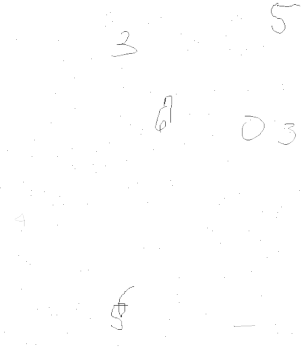
\includegraphics[width=1.37569in,height=1.575in,alt={image\_90007}]{./media_en/media/image5.png}

Figure 3.4 Sample images generated by v1 &
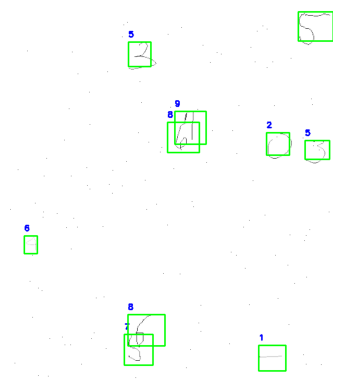
\includegraphics[width=1.38472in,height=1.575in,alt={ }]{./media_en/media/image6.png}

Figure 3.5 Sample annotated by v1 \\
\end{longtable}
}

\begin{enumerate}
\def\labelenumi{\arabic{enumi}.}
\setcounter{enumi}{2}
\item
  v2
\end{enumerate}

\begin{quote}
The following adjustments have been made to address the problems
encountered in v1:

-Change the logic of random point generation. Instead of directly adding
images from the list and placing them randomly, n points are generated
randomly first to ensure the interval between these n points, and then
these n points are positioned as the upper left point of the image to
avoid repeated images.

-Rewrote the alpha channel generation method to reduce the threshold for
removing white backgrounds and prevent elements from having too few
features.

V2 has been able to generate basic multi-element data sets stably, and
continue to generate matrices and elements in the matrices, so that
features are more diversified and generalized. This is achieved by
adaptive splicing after generating matrix elements.

Generation of matrix elements: According to the actual situation, 1-3
digits are generated. When the number of bits is\textgreater2, the first
digit has a probability of being negative, and the size and interval of
appropriate random numbers are arranged.

Generation matrix: An algorithm for adjusting the size of images
according to the number of adaptive elements and an algorithm for
placing matrix elements according to the number of adaptive rows and
columns are written.
\end{quote}

{\def\LTcaptype{none} % do not increment counter
\begin{longtable}[]{@{}
  >{\centering\arraybackslash}p{(\linewidth - 2\tabcolsep) * \real{0.5000}}
  >{\centering\arraybackslash}p{(\linewidth - 2\tabcolsep) * \real{0.5000}}@{}}
\toprule\noalign{}
\endhead
\bottomrule\noalign{}
\endlastfoot
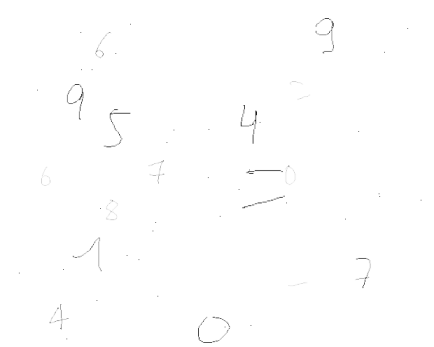
\includegraphics[width=1.97222in,height=1.575in,alt={alpha\_50001}]{./media_en/media/image7.png}

Figure 3.6 Example of alpha pattern generated by v2 &
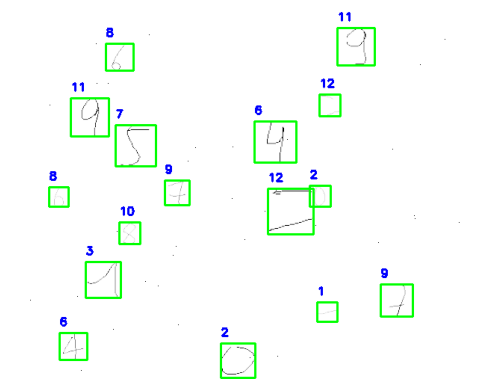
\includegraphics[width=1.95139in,height=1.575in,alt={ }]{./media_en/media/image8.png}

Figure 3.7 Sample alpha annotation generated by v2 \\
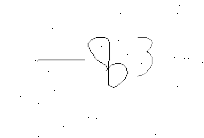
\includegraphics[width=1.96875in,height=1.33194in,alt={horizontal\_57756}]{./media_en/media/image9.png}

Figure 3.8 Matrix element pattern generated by v2 &
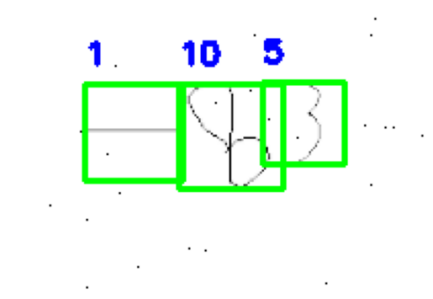
\includegraphics[width=1.96875in,height=1.35694in,alt={  }]{./media_en/media/image10.png}

Figure 3.9 Sample matrix element labeling generated by v2 \\
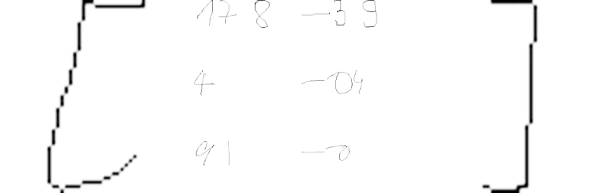
\includegraphics[width=2.75625in,height=0.87639in,alt={matrix\_59157}]{./media_en/media/image11.png}

Figure 3.10 Matrix pattern generated by v2 &
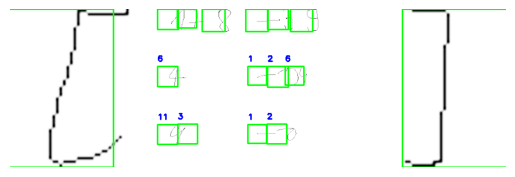
\includegraphics[width=2.75625in,height=0.94722in,alt={ }]{./media_en/media/image12.png}

Figure 3.11 Sample matrix annotations generated by v2 \\
\end{longtable}
}

\begin{enumerate}
\def\labelenumi{\arabic{enumi}.}
\setcounter{enumi}{3}
\item
  v3
\end{enumerate}

\begin{quote}
The following adjustments have been made to address the problems
encountered in version v2:

-Fix the misalignment of labels in version v2.

-Adjust the adaptive vertical stretching relationship of the left and
right brackets of the matrix, and randomly move up, down, left and right
to mimic the matrix written by hand.

-An adaptive centering algorithm for elements in the matrix is added to
prepare for subsequent clustering and segmentation, which more imitates
the characteristics of handwritten matrices.
\end{quote}

{\def\LTcaptype{none} % do not increment counter
\begin{longtable}[]{@{}
  >{\centering\arraybackslash}p{(\linewidth - 2\tabcolsep) * \real{0.5082}}
  >{\centering\arraybackslash}p{(\linewidth - 2\tabcolsep) * \real{0.4918}}@{}}
\toprule\noalign{}
\endhead
\bottomrule\noalign{}
\endlastfoot
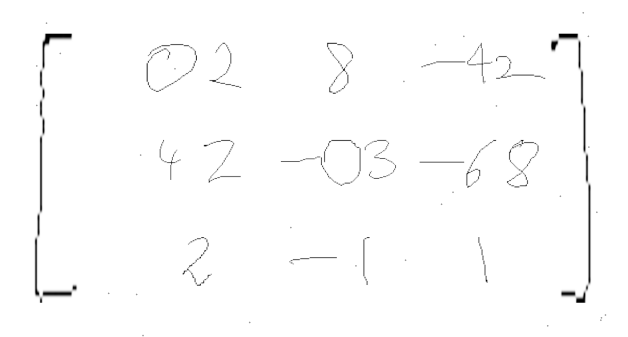
\includegraphics[width=2.85625in,height=1.53125in,alt={matrix\_90048}]{./media_en/media/image13.png}

Figure 3.12 Matrix pattern generated by v3 &
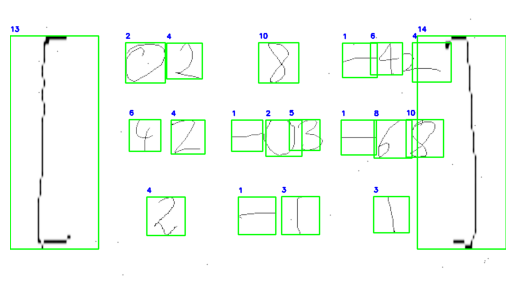
\includegraphics[width=2.75625in,height=1.53056in,alt={ }]{./media_en/media/image14.png}

Figure 3.13 Matrix annotation sample generated by v3 \\
\end{longtable}
}

\begin{enumerate}
\def\labelenumi{\arabic{enumi}.}
\setcounter{enumi}{4}
\item
  v4
\end{enumerate}

\begin{quote}
The following adjustments have been made to address the problems
encountered in v3:

-Adjust the thickness of elements in the matrix, adjust the generation
logic of alpha elements, and add the alpha channel when adding elements
to the matrix.

-Adjust the noise generation logic. The noise is now gradually
decreasing from the center to the surrounding alpha value, mimicking the
actual image preprocessing noise.

-The matrix adaptive position centering, row and column positions,
spacing and other features have been optimized. Now the matrix is very
close to the handwritten matrix.
\end{quote}

{\def\LTcaptype{none} % do not increment counter
\begin{longtable}[]{@{}
  >{\centering\arraybackslash}p{(\linewidth - 2\tabcolsep) * \real{0.5000}}
  >{\centering\arraybackslash}p{(\linewidth - 2\tabcolsep) * \real{0.5000}}@{}}
\toprule\noalign{}
\endhead
\bottomrule\noalign{}
\endlastfoot
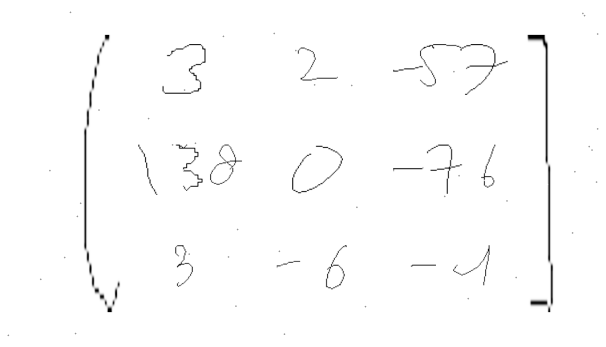
\includegraphics[width=2.75625in,height=1.57569in,alt={matrix\_94875}]{./media_en/media/image15.png}

Figure 3.14 Matrix pattern generated by v4 &
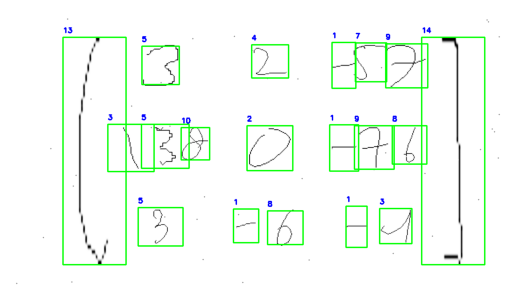
\includegraphics[width=2.67639in,height=1.575in,alt={ }]{./media_en/media/image16.png}

Figure 3.15 Example of matrix annotation generated by v4 \\
\end{longtable}
}

Through the optimization and adjustment of the matrix generation
algorithm by multiple iterations, the final stable version of the matrix
automatic generation and annotation data set was obtained, and the model
training was entered, with a total of 300,000 images. The ratio of the
training set to the test set was 9:1, and the sample of the data set is
shown in Figure 3.16.

\begin{figure}
\centering
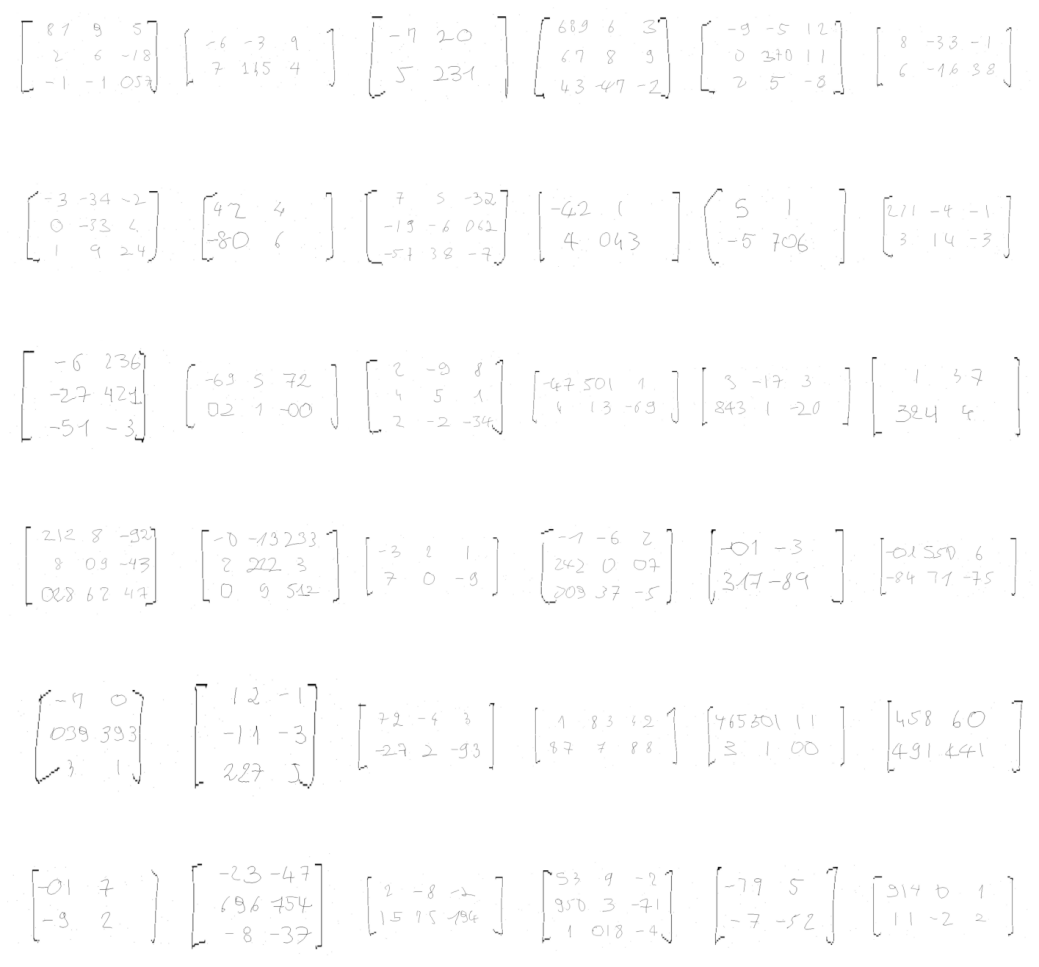
\includegraphics[width=4.72441in,height=4.39465in,alt={,  }]{./media_en/media/image17.png}
\caption{Figure 3.16 Sample graph of generated data set}
\end{figure}

The algorithm flowchart of the final stable version is shown in Figure
3.17, and the specific code is shown in Appendix I Algorithm 1.

\begin{figure}
\centering
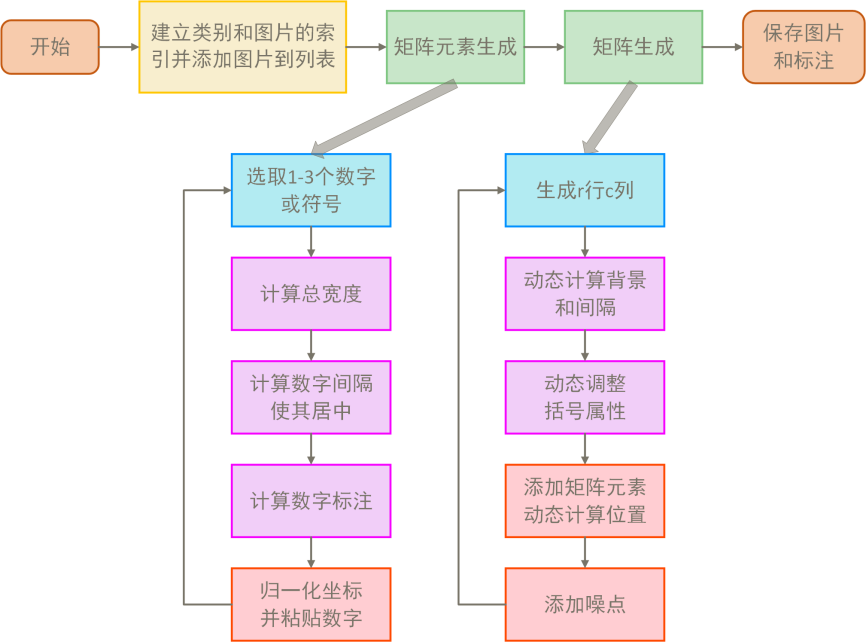
\includegraphics[width=3.93681in,height=2.91597in,alt={}]{./media_en/media/image18.png}
\caption{Figure 3.17 Flowchart of the data generation algorithm}
\end{figure}

\section{Key methods}\label{key-methods}

\subsection{Mathematical equation
detection}\label{mathematical-equation-detection}

\subsubsection{Mathematical equation model
training}\label{mathematical-equation-model-training}

In terms of network architecture and model training, this project
selected the lightweight YOLOv11n as the basic object detection
framework. It performed dual optimization at both structural and
mechanism levels based on the spatial distribution characteristics of
handwritten equation images. Due to the integration of YOLO, Mamba, and
CoordAttention modules, I refer to the network as YMCANet in the
following text. The network architecture is divided into three major
modules: Backbone, Neck, and Head.

Layer Backbone builds upon the existing C2F structure by incorporating a
more expressive C3K2 multi-scale convolution module, significantly
enhancing the ability to capture complex edges and stroke features. To
further boost network performance, a Mamba backbone network is
introduced, improving the overall expressive power and computational
efficiency of the model. Additionally, VSS, VCM, and XSS modules are
added to the network, effectively enhancing the fusion capability of
multi-scale information and the accuracy of feature extraction.

In terms of attention mechanism, the original PSA module is optimized
and replaced with CoordAttention coordinate attention mechanism{[}7{]},
so that the network can not only pay attention to content information
when recognizing the matrix, but also grasp the spatial position of
characters in the image more accurately, thus improving the recognition
accuracy and robustness.

\begin{enumerate}
\def\labelenumi{\arabic{enumi}.}
\item
  VSS Visual State Space Module
\end{enumerate}

The VSS module effectively models visual elements in images by
introducing a visual state space. In traditional visual recognition
tasks, information in images is typically static. However, in VSS, each
visual element is treated as a dynamic state that can change during
image processing. This module captures dynamic information at different
levels of visual data, such as changes in objects, background
variations, and the relationships between visual elements.

\begin{enumerate}
\def\labelenumi{\arabic{enumi}.}
\setcounter{enumi}{1}
\item
  VCM convolution feature fusion module
\end{enumerate}

The VCM module is primarily used to integrate feature information from
different convolutional layers, enhancing the network\textquotesingle s
ability to understand complex image features. It achieves this by
weighting and fusing the output features from multiple convolutional
layers, ensuring that the network can effectively combine information at
different levels, thus increasing the diversity and depth of feature
representation. VCM enables the network to better handle image
information with varying scales and resolutions, thereby improving the
accuracy of feature extraction, especially when dealing with complex
scenes or images.

\begin{enumerate}
\def\labelenumi{\arabic{enumi}.}
\setcounter{enumi}{2}
\item
  The XSS extension receptive field module
\end{enumerate}

The XSS module, by expanding the receptive field of convolutional
kernels, can capture a broader range of contextual information. This
module leverages multi-layer convolution operations to effectively
extend the network\textquotesingle s perception of distant pixels in
images, making the model more accurate when processing features over
large areas. The XSS module has strong capabilities in capturing
long-range dependencies and complex backgrounds in images, enhancing the
network\textquotesingle s performance in multi-scale feature fusion,
especially in scenarios with high image resolution or complex
structures.

\begin{enumerate}
\def\labelenumi{\arabic{enumi}.}
\setcounter{enumi}{3}
\item
  CoordAttention Coordinate attention mechanism
\end{enumerate}

CoordAttention is an attention mechanism based on spatial coordinates.
Unlike traditional channel attention mechanisms, it not only focuses on
content information in the image but also introduces coordinate
information to accurately grasp the spatial position of characters
within the image. By weighting the coordinates, CoordAttention can make
the network more focused on key areas, enhancing its ability to
understand spatial structure and layout. When recognizing matrices,
CoordAttention can accurately locate the specific positions and shapes
of characters, thereby improving recognition accuracy and robustness,
especially in complex backgrounds or when characters are distorted.

\begin{figure}
\centering
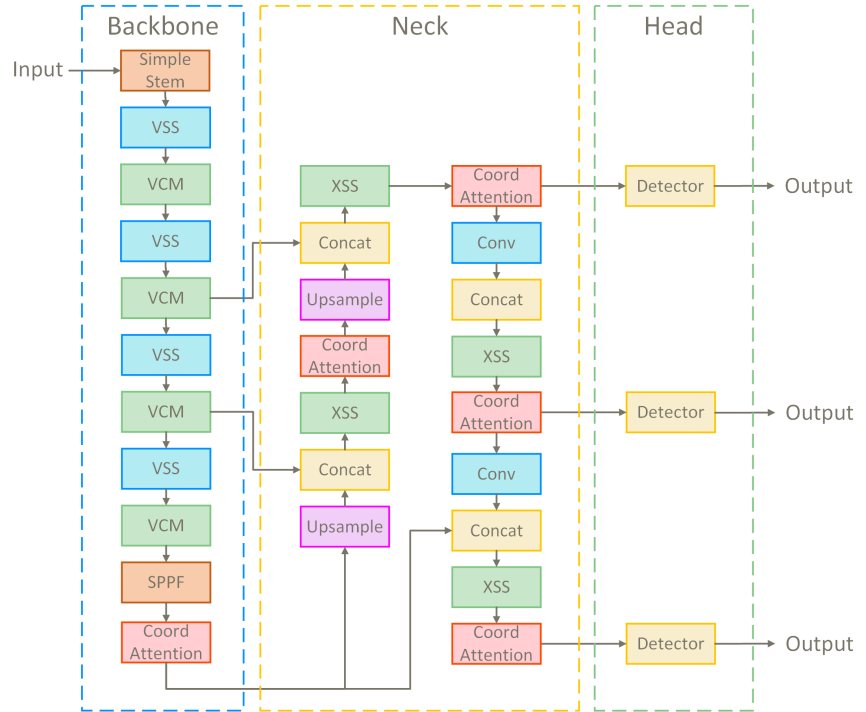
\includegraphics[width=3.93681in,height=3.23542in,alt={yolo-mamba}]{./media_en/media/image19.png}
\caption{Figure 4.1 YMCANet Network model diagram}
\end{figure}

CoordAttention The coordinate attention mechanism can capture the
spatial relationship of a specific location and make use of it in the
attention calculation. The algorithm flow chart is shown in Figure 3.6.

\begin{figure}
\centering
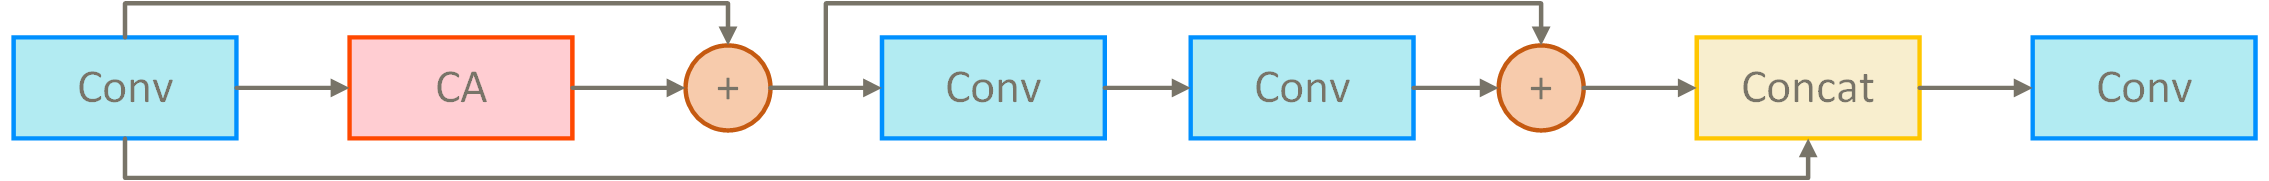
\includegraphics[width=5.51181in,height=0.43958in,alt={CA}]{./media_en/media/image20.png}
\caption{Figure 4.2 CoordAttention Module algorithm flow chart}
\end{figure}

Algorithm calculation formula:

\begin{longtable}[]{@{}
  >{\centering\arraybackslash}p{(\linewidth - 6\tabcolsep) * \real{0.2900}}
  >{\centering\arraybackslash}p{(\linewidth - 6\tabcolsep) * \real{0.3550}}
  >{\centering\arraybackslash}p{(\linewidth - 6\tabcolsep) * \real{0.2316}}
  >{\centering\arraybackslash}p{(\linewidth - 6\tabcolsep) * \real{0.1006}}@{}}
\caption{Figure 4.3 Comparison of attention module
effects}\tabularnewline
\toprule\noalign{}
\endfirsthead
\endhead
\bottomrule\noalign{}
\endlastfoot
\multicolumn{3}{@{}>{\centering\arraybackslash}p{(\linewidth - 6\tabcolsep) * \real{0.8766} + 4\tabcolsep}}{%
\(output = \ Conv1 \times 1(concat(a\ ,\  + \ Cooratt(b)\  + \ FFN(b)))\)}
& (1) \\
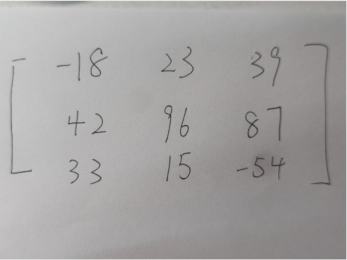
\includegraphics[width=1.575in,height=1.18403in,alt={ }]{./media_en/media/image21.png}

artwork master &
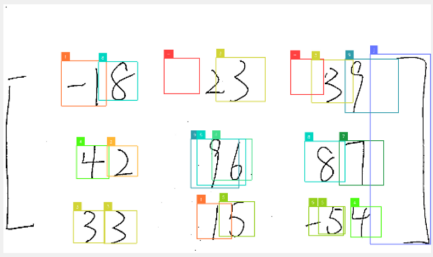
\includegraphics[width=1.96875in,height=1.16667in,alt={ }]{./media_en/media/image22.png}

PSA module &
\multicolumn{2}{>{\centering\arraybackslash}p{(\linewidth - 6\tabcolsep) * \real{0.3322} + 2\tabcolsep}@{}}{%
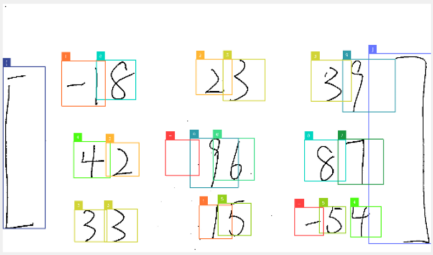
\includegraphics[width=1.96875in,height=1.16042in,alt={ }]{./media_en/media/image23.png}

CA module} \\
\end{longtable}

The training phase utilized a self-developed handwriting matrix dataset
(comprising 300,000 images with various arrangements and interference
forms). Within 10 rounds of training, the model achieved an accuracy
above maP500.95, demonstrating excellent convergence speed and
generalization ability. Additionally, the training process involved
pre-training transfer between multiple generations of models, combined
with fine-tuning and hierarchical visualization, effectively enhancing
the model\textquotesingle s recognition stability under complex writing
styles, providing a solid foundation for subsequent step-by-step visual
computation.

{\def\LTcaptype{none} % do not increment counter
\begin{longtable}[]{@{}
  >{\raggedright\arraybackslash}p{(\linewidth - 2\tabcolsep) * \real{0.4485}}
  >{\centering\arraybackslash}p{(\linewidth - 2\tabcolsep) * \real{0.5515}}@{}}
\toprule\noalign{}
\endhead
\bottomrule\noalign{}
\endlastfoot
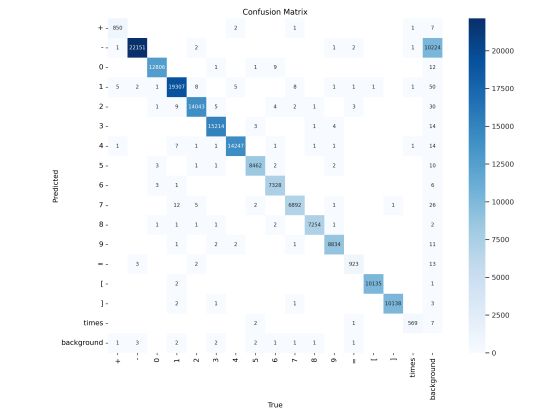
\includegraphics[width=2.6125in,height=2.08472in,alt={confusion\_matrix}]{./media_en/media/image24.png}

Figure 4.4 Matrix pattern generated by v4 &
F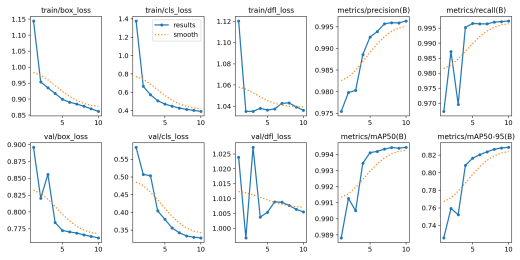
\includegraphics[width=3.25486in,height=2.09792in,alt={results}]{./media_en/media/image25.png}igure
4.5 Examples of matrix annotations generated by v4 \\
\end{longtable}
}

\subsubsection{Formula image
preprocessing}\label{formula-image-preprocessing}

Since the generated data set is binary, it is necessary to carry out
image preprocessing algorithm and appropriate scaling preprocessing for
the input captured image. The specific algorithm flow chart is shown in
Figure 3.10.

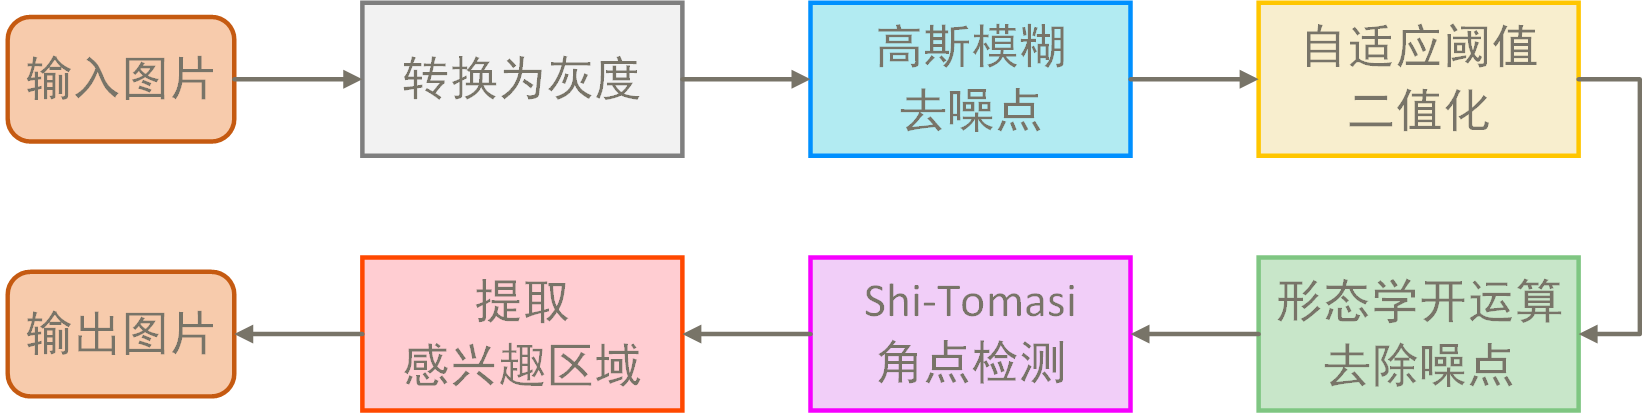
\includegraphics[width=4.52847in,height=1.13333in,alt={}]{./media_en/media/image26.png}

Figure 4.6 Flow chart of image preprocessing algorithm

(1) Convert to grayscale image and Gaussian blur denoising:

Application cv2.GaussianBlur smooths the image. By using a 5x5 Gaussian
kernel through convolution operations, the image is blurred, with the
standard deviation automatically calculated based on the kernel size.
This process can smooth the image, remove fine noise, making subsequent
thresholding and morphological processing more accurate and reliable.
The specific formula for the operation is as follows:

{\def\LTcaptype{none} % do not increment counter
\begin{longtable}[]{@{}
  >{\centering\arraybackslash}p{(\linewidth - 2\tabcolsep) * \real{0.9399}}
  >{\centering\arraybackslash}p{(\linewidth - 2\tabcolsep) * \real{0.0601}}@{}}
\toprule\noalign{}
\endhead
\bottomrule\noalign{}
\endlastfoot
\(I_{\text{blurred}}(x,y) = \sum_{i = - k}^{k}{\sum_{j = - k}^{k}{I(x + i,y + j)K(i,j)}}\)
& (2) \\
\end{longtable}
}

(2) Adaptive threshold processing:

Binary image processing is used to retain only black and white pixels,
making it easier to distinguish between foreground and background. The
cv2.adaptiveThreshold method is employed, automatically adjusting the
threshold based on the brightness of the surrounding area of each pixel,
effectively addressing uneven lighting conditions. The
cv2.ADAPTIVE\_THRESH\_GAUSSIAN\_C method is utilized, where the weighted
average of pixels within a neighborhood serves as the local threshold,
thus adapting to images under various lighting conditions. The specific
formula for adaptive threshold calculation is as follows:

{\def\LTcaptype{none} % do not increment counter
\begin{longtable}[]{@{}
  >{\raggedright\arraybackslash}p{(\linewidth - 2\tabcolsep) * \real{0.9399}}
  >{\centering\arraybackslash}p{(\linewidth - 2\tabcolsep) * \real{0.0601}}@{}}
\toprule\noalign{}
\endhead
\bottomrule\noalign{}
\endlastfoot
\(T(x,y) = \frac{1}{N}\sum_{i = - \left\lfloor \frac{N}{2} \right\rfloor}^{\left\lfloor \frac{N}{2} \right\rfloor}{\sum_{j = - \left\lfloor \frac{N}{2} \right\rfloor}^{\left\lfloor \frac{N}{2} \right\rfloor}{I(x + i,y + j)}}\)
& (3) \\
\end{longtable}
}

(3) Morphological open operation to remove noise:

Clean up small noise points in the image and enhance the connectivity of
the target area. An opening operation was used, first erosion followed
by dilation, to remove small white noise points. The cv2.morphologyEx
function with a cv2.MORPH\_RECT rectangular structuring element was
applied to the image to improve the effectiveness of subsequent corner
detection. The specific formula for the operation is as follows.

Corrosion operation:

{\def\LTcaptype{none} % do not increment counter
\begin{longtable}[]{@{}
  >{\raggedright\arraybackslash}p{(\linewidth - 2\tabcolsep) * \real{0.9399}}
  >{\centering\arraybackslash}p{(\linewidth - 2\tabcolsep) * \real{0.0601}}@{}}
\toprule\noalign{}
\endhead
\bottomrule\noalign{}
\endlastfoot
\(E(x,y) = \min_{(i,j) \in S}I(x + i,y + j)\) & (4) \\
\end{longtable}
}

expansive working:

{\def\LTcaptype{none} % do not increment counter
\begin{longtable}[]{@{}
  >{\raggedright\arraybackslash}p{(\linewidth - 2\tabcolsep) * \real{0.9399}}
  >{\centering\arraybackslash}p{(\linewidth - 2\tabcolsep) * \real{0.0601}}@{}}
\toprule\noalign{}
\endhead
\bottomrule\noalign{}
\endlastfoot
\(D(x,y) = \max_{(i,j) \in S}E(x + i,y + j)\) & (5) \\
\end{longtable}
}

(4) Shi-Tomasi corner detection:

The Shi-Tomasi corner detection algorithm cv2.goodFeaturesToTrack was
used to detect areas of intense change in images, improving accuracy
compared to commonly used Harris and Fast clustering methods, and adding
the selection of optimal corners. The maximum number of corners
extracted is limited to 100, with higher quality corners being selected.
Corner detection provides positional information for target areas,
aiding subsequent steps in more accurately extracting regions of
interest. The formula for the gradient covariance matrix of each
pixel\textquotesingle s neighborhood is as follows:

{\def\LTcaptype{none} % do not increment counter
\begin{longtable}[]{@{}
  >{\centering\arraybackslash}p{(\linewidth - 2\tabcolsep) * \real{0.9399}}
  >{\centering\arraybackslash}p{(\linewidth - 2\tabcolsep) * \real{0.0601}}@{}}
\toprule\noalign{}
\endhead
\bottomrule\noalign{}
\endlastfoot
\(M\  = \ \begin{bmatrix}
\sum I_{x}^{2} & \sum I_{x}I_{y} \\
\sum I_{x}I_{y} & \sum I_{y}^{2}
\end{bmatrix}\) & (6) \\
\end{longtable}
}

(5) Boundary range calculation and interest area extraction and
transformation:

The minimum and maximum boundaries of the region of interest are
calculated from the extracted corner coordinates, and the edge offset is
further ensured that these boundaries do not exceed the actual range of
the image. The extracted slices are returned as a color image.

The final results of preprocessing are shown in Figure 4.7.

{\def\LTcaptype{none} % do not increment counter
\begin{longtable}[]{@{}
  >{\raggedright\arraybackslash}p{(\linewidth - 2\tabcolsep) * \real{0.3897}}
  >{\raggedright\arraybackslash}p{(\linewidth - 2\tabcolsep) * \real{0.3539}}@{}}
\toprule\noalign{}
\endhead
\bottomrule\noalign{}
\endlastfoot
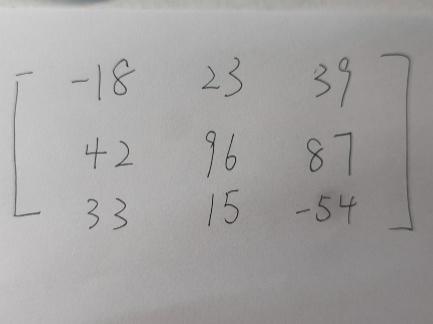
\includegraphics[width=1.9625in,height=0.99931in,alt={ }]{./media_en/media/image27.jpeg}

artwork master &
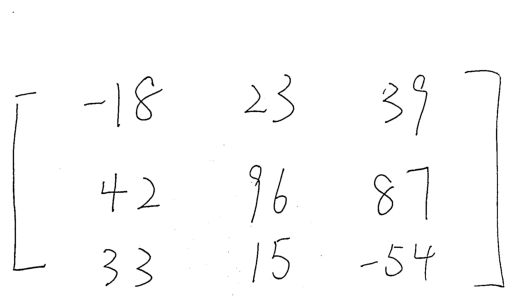
\includegraphics[width=1.96736in,height=0.96458in,alt={ }]{./media_en/media/image28.png}

Preprocessing results \\
\end{longtable}
}

Figure 4.7 Preprocessing results

\subsubsection{Formula content
detection}\label{formula-content-detection}

In the content detection module of the algorithm, the system calls the
YOLOv11 model provided by ultralytics and uses the supervision library
to uniformly monitor and process the detection results. It mainly
returns the center coordinates, width and height, as well as category
annotations for each recognition box. To improve recognition accuracy
and avoid duplicate recognition issues, the system introduces a
deduplication mask mechanism based on IoU (Intersection over Union). By
calculating the overlap ratio between two detection boxes, it filters
out redundant detection results with low confidence, effectively
reducing the risk of overfitting. Additionally, the system generates
masks for each element, providing spatial foundations for subsequent
DBSCAN clustering segmentation and matrix structure reconstruction. This
module not only ensures precise localization of handwritten characters
but also lays a solid data foundation for the structural recognition and
visual computation of the entire matrix.

The system also adds a return value to return all the annotated masks,
which is ready for subsequent clustering segmentation. The processing
results are shown in Figure 4.8.

{\def\LTcaptype{none} % do not increment counter
\begin{longtable}[]{@{}
  >{\centering\arraybackslash}p{(\linewidth - 2\tabcolsep) * \real{0.5000}}
  >{\centering\arraybackslash}p{(\linewidth - 2\tabcolsep) * \real{0.5000}}@{}}
\toprule\noalign{}
\endhead
\bottomrule\noalign{}
\endlastfoot
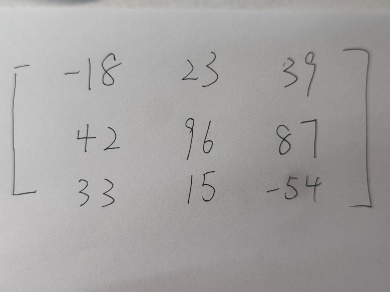
\includegraphics[width=2.05486in,height=1.29861in]{./media_en/media/image29.jpeg}

artwork master &
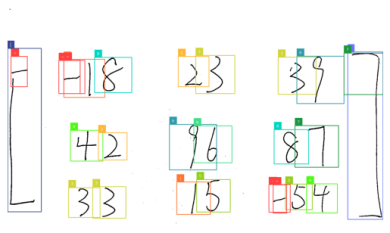
\includegraphics[width=1.96806in,height=1.17639in,alt={ }]{./media_en/media/image30.png}

Preprocessing results \\
\end{longtable}
}

Figure 4.8 Yolo detection results

\subsubsection{Mathematical formula number
extraction}\label{mathematical-formula-number-extraction}

After receiving the return value of 4.1.3 detection, cluster and segment
the matrix to determine its row and column numbers. Then draw the
segmentation lines to prepare for determining which area each individual
number symbol belongs to in the future. Finally, return a list of
horizontal and vertical segmentation lines. The algorithm flowchart is
shown in Figure 4.9.

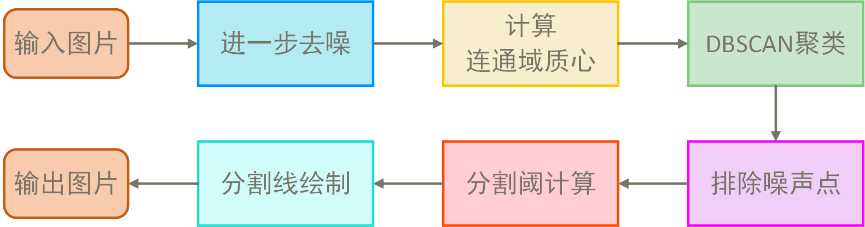
\includegraphics[width=3.93681in,height=1.02986in,alt={ }]{./media_en/media/image31.png}

Figure 4.9 Flow chart of clustering segmentation algorithm

Using cv2.findContours to find connected regions in images, the centroid
of these regions is calculated through cv2.moments image moments. Given
a point p and radius ϵ, if there are enough neighboring points within
this radius, these points are considered to belong to the
\((cX,cY)\)same cluster. Based on the number of centroids, the initial
calculation of the row and column numbers of the region grid is
performed. For each centroid, its associated rectangular area is
calculated. Multiple segmentation lines are drawn using the intersection
points of clustered regions, and then the segmentation lines are
filtered using deduplication operations.

The line validation checks whether there is a centroid on both sides of
a certain line. If not, this line is excluded to ensure that each line
indeed serves as a row or column division in the matrix. Ultimately, two
lists are obtained: horizontal and vertical lines, which are then
returned to the number extraction module. The result is shown in Figure
4.10.

{\def\LTcaptype{none} % do not increment counter
\begin{longtable}[]{@{}
  >{\raggedright\arraybackslash}p{(\linewidth - 2\tabcolsep) * \real{0.4576}}
  >{\centering\arraybackslash}p{(\linewidth - 2\tabcolsep) * \real{0.5000}}@{}}
\toprule\noalign{}
\endhead
\bottomrule\noalign{}
\endlastfoot
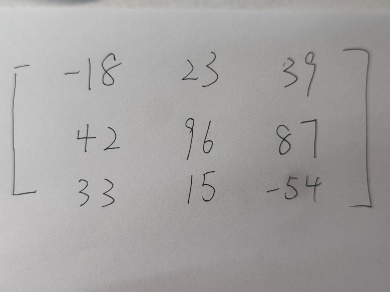
\includegraphics[width=2.47917in,height=1.44236in,alt={ }]{./media_en/media/image29.jpeg}

artwork master &
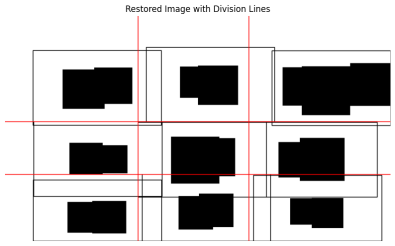
\includegraphics[width=2.40139in,height=1.49097in,alt={ }]{./media_en/media/image32.png}

Preprocessing results \\
\end{longtable}
}

Figure 4.10 Results of clustering segmentation algorithm

First, through normalization operations, we determine the exact relative
positions of each element. To ensure that the original positional
relationships remain unchanged when placing corresponding elements in
each row and column, we sort the x\_center values of each element and
add them to a list. Traverse the entire list, and based on the relative
positional relationships between elements x\_center and y\_center with
respect to the partition lines returned by the clustering segmentation
algorithm in Figure 4.10, place the elements in their corresponding
positions. After concatenating the strings, perform type conversion to
return an array format of numpy for easier Latex presentation later. The
result is shown in 4.11.

{\def\LTcaptype{none} % do not increment counter
\begin{longtable}[]{@{}
  >{\centering\arraybackslash}p{(\linewidth - 4\tabcolsep) * \real{0.3012}}
  >{\centering\arraybackslash}p{(\linewidth - 4\tabcolsep) * \real{0.3360}}
  >{\centering\arraybackslash}p{(\linewidth - 4\tabcolsep) * \real{0.3391}}@{}}
\toprule\noalign{}
\endhead
\bottomrule\noalign{}
\endlastfoot
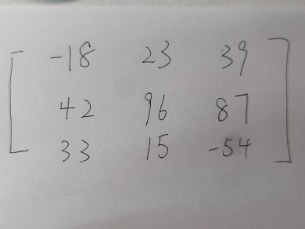
\includegraphics[width=1.57431in,height=1.17986in,alt={ }]{./media_en/media/image33.jpeg}

artwork master &
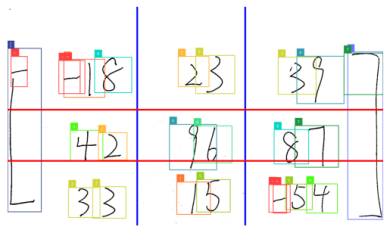
\includegraphics[width=1.77153in,height=1.05903in,alt={ }]{./media_en/media/image34.png}

Split line results &

\includegraphics[width=1.77153in,height=0.99653in,alt={ }]{./media_en/media/image35.png}

Latex matrix display \\
\end{longtable}
}

Figure 4.11 Digital extraction results

\subsection{Step-by-step solution animation
module}\label{step-by-step-solution-animation-module}

In terms of animation module construction, the system carries out
underlying graphics rendering based on the mathematical visualization
engine Manim of Python, and completes frame-by-frame video output
combined with ffmpeg, realizing dynamic visualization demonstration of
matrix operation process.

By inheriting the basic graphic objects and text classes from Manim, a
custom class SquTex was constructed. This class encapsulates the
combination of squares and text for each matrix element, enabling
absolute position control, format style adjustment, and animation
presentation of individual elements. Subsequently, based on SquTex, a
MatrixCal class was designed to achieve logical expression and layout
control of two-dimensional matrix objects, supporting high-precision
positioning and bracket labeling for each element. At the computational
level, a MatrixDet class was developed for determinant calculations,
supporting the extraction of multiplication paths from the main and
secondary diagonals and calculating intermediate values. The
encapsulated animation methods are called to display each group of
multiplication and addition processes in a diagonal manner, highlighting
key paths and the logic of result derivation. For matrix addition and
multiplication, the MatrixMath class introduces a dual-input structure,
using two original matrices as input objects for sequential operations.
It achieves element-by-element alignment for addition and item-by-item
expansion for multiplication through constructing progress vectors and
calculating annotation texts. This enhances the transparency and
interpretability of the calculation process. The entire animation system
adopts a modular design, with clear inheritance and independent
functional units, ensuring scalability and reusability. It is a core
supporting component that professionally and dynamically presents
abstract mathematical computation logic, as shown in Figure 4.12.

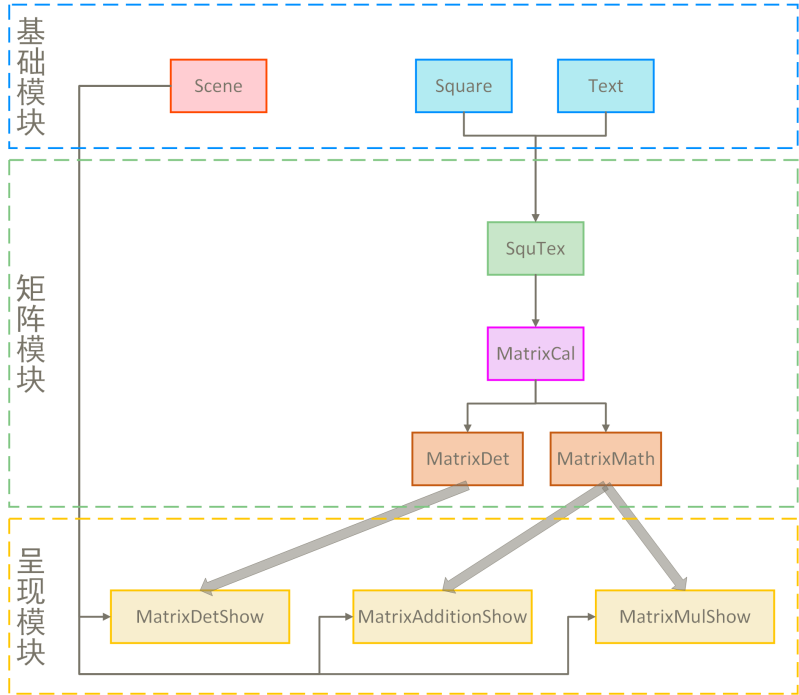
\includegraphics[width=4.03472in,height=3.5125in,alt={}]{./media_en/media/image36.png}

Figure 4.12 Animation module class object inheritance diagram

\subsubsection{Step-by-step solution frame by frame rendering
method}\label{step-by-step-solution-frame-by-frame-rendering-method}

The Manim engine provides a complete vector animation scene management
system by inheriting from Scene or ThreeDScene. This project uses the
construct() function as the main entry point for animations, where
graphic objects and animation control commands are gradually called to
achieve dynamic computation demonstrations. All rendering results are
generated at the frame level using vector graphics (SVG), and ultimately
synthesized and encoded through ffmpeg for high-quality MP4 video
output. This mechanism offers excellent resolution scalability and
smooth animation, meeting the visualization requirements of highly
complex mathematical expressions.

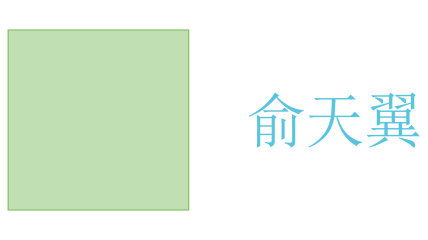
\includegraphics[width=3.64583in,height=2.04722in,alt={ }]{./media_en/media/image37.png}

Figure 4.13 Example of a basic module

\subsubsection{The control scheme for each animation
element}\label{the-control-scheme-for-each-animation-element}

By inheriting the and classes shown in the basic \(SquareText\)module of
Figure 2, define an element as a group of squares and text. When
creating the structure, input a list or string as a variable parameter
to create a list of square text combinations. The specific construction
function is shown in Code 1.

Code 1 SquTex Constructor

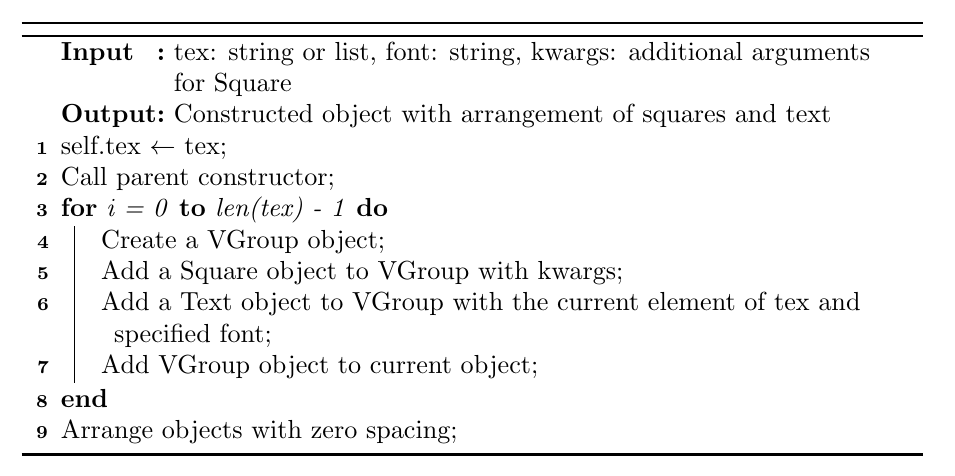
\includegraphics[width=3.93681in,height=1.96181in,alt={ }]{./media_en/media/image38.png}

The SquTex is a fundamental graphic composite class in the animation
system. By inheriting from the Manim\textquotesingle s VGroup object, it
models each mathematical element as a "square border + text" composite
structure, featuring high-precision position management and style
control capabilities. During the construction phase, it can accept a
list of strings and automatically generate a set of orderly arranged
graphic units. This class integrates methods such as position sorting,
symbol addition, style modification, and unit animation grouping,
supporting the positioning, highlighting, bolding, and style switching
of any element in the matrix. Through encapsulation of animation
interfaces like animate\_one\_by\_one() and add\_bracket(), it achieves
frame-by-frame control and diverse visual effects during the matrix
presentation process. The specific effects are shown in Figure 4.14.

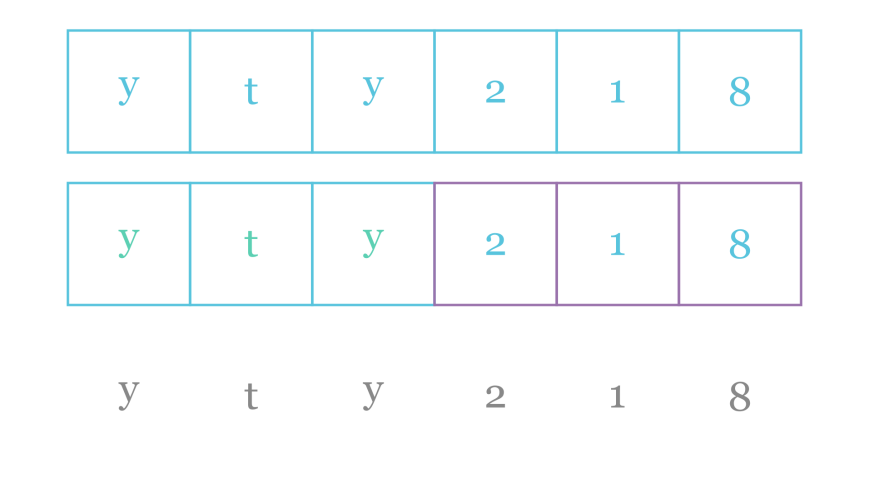
\includegraphics[width=3.64514in,height=2.04583in,alt={  }]{./media_en/media/image39.png}

Figure 4.14 SquTex Example diagram

\subsubsection{Build basic formula animation
class}\label{build-basic-formula-animation-class}

To meet the dynamic visualization needs for determinant calculations, a
class called MatrixDet has been constructed. This class inherits from
the base matrix structure class MatrixCal and further extends with
specialized logic for visual demonstrations. Not only does it support
precise extraction of element paths along the main diagonal and
secondary diagonal, but it also automatically calculates and renders the
intermediate values of each multiplication path, visually highlighting
each element involved in the computation one by one. Through color
coding, path animations, and numerical annotations, it dynamically
presents the process of expanding determinants. The system can
automatically generate corresponding calculation expressions (such as
a11 × a22 × a33 +...), merge positive and negative terms visually, and
ultimately output clear and complete dynamic expansion animations.

Code 2 MatrixCal Constructor

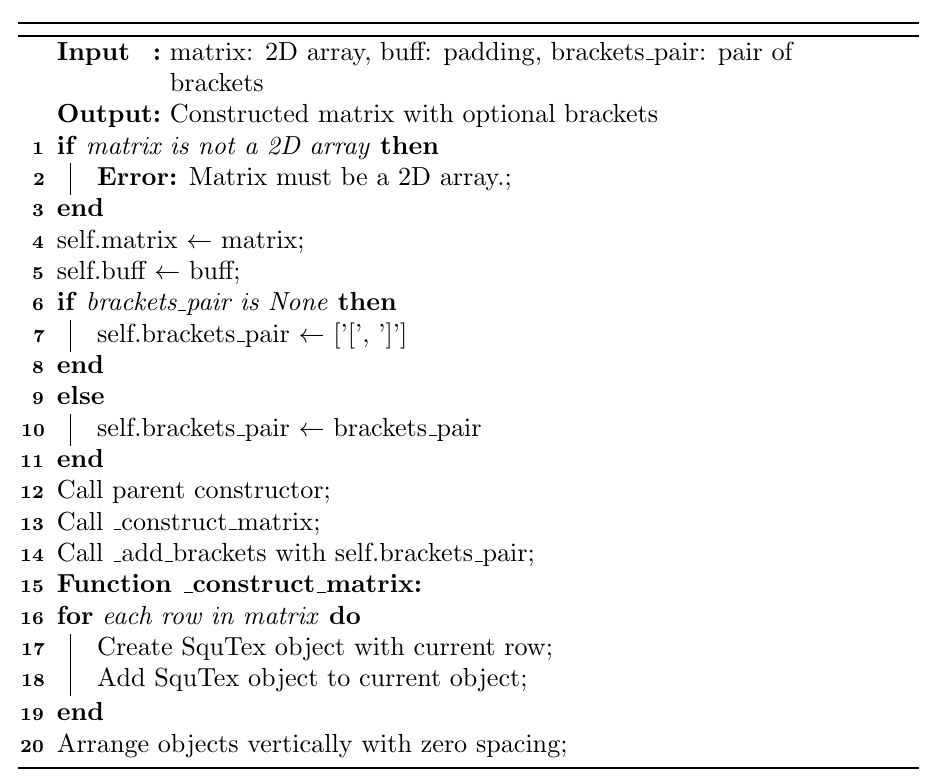
\includegraphics[width=3.33819in,height=2.77222in,alt={ }]{./media_en/media/image40.png}

This class extracts the set of elements involved in a multiplication
step through the get\_process\_inform() method and records their product
value accordingly; it then calls cal\_progress\_times() to generate a
visual expression with an equal sign and a multiplication symbol. The
final cal\_result\_addition() function integrates all process results,
dynamically generating addition and subtraction expressions along with
the final value. This class works in conjunction with a unified timeline
animation control logic to fully reproduce the entire process from
element selection to calculation results of determinants. The specific
effect is shown in Figure 4.15.

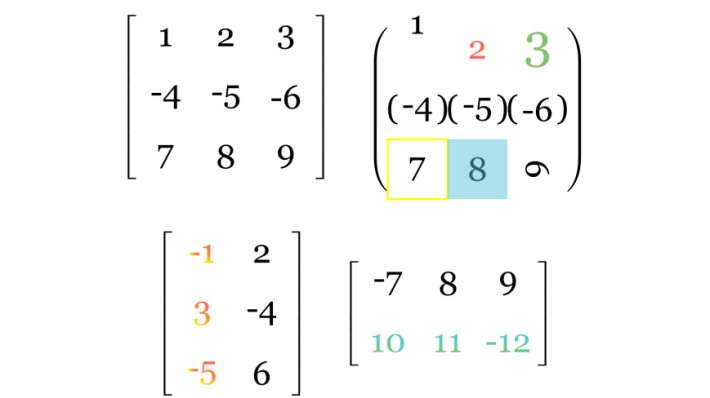
\includegraphics[width=3.22639in,height=1.81042in,alt={ }]{./media_en/media/image41.png}

Figure 4.15 MatrixCal Example diagram

\subsubsection{Monocular operation is divided into step-by-step
animation
construction}\label{monocular-operation-is-divided-into-step-by-step-animation-construction}

In view of the dynamic visualization requirements for determinant
calculation, a class MatrixDet is constructed, which inherits from
MatrixCal and adds the functions of extracting the product path of the
main diagonal and the secondary diagonal and visualizing the
intermediate process.

Code 3 MatrixDet Constructor

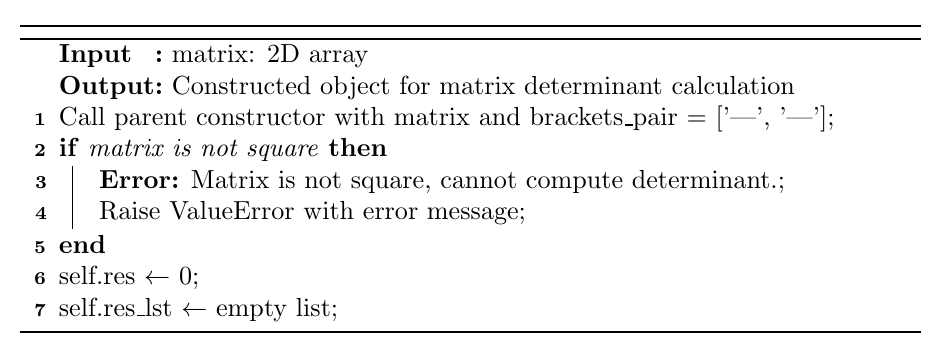
\includegraphics[width=3.87569in,height=1.45139in,alt={ }]{./media_en/media/image42.png}

This class extracts the set of elements involved in a multiplication
step through the get\_process\_inform() method and records their product
value accordingly; it then calls cal\_progress\_times() to generate a
visual expression with an equal sign and a multiplication symbol. The
final cal\_result\_addition() function integrates all process results,
dynamically generating addition and subtraction expressions along with
the final value. This class works in conjunction with a unified timeline
animation control logic to fully reproduce the entire process from
element selection to calculation results of determinants. The specific
effect is shown in Figure 3.16.

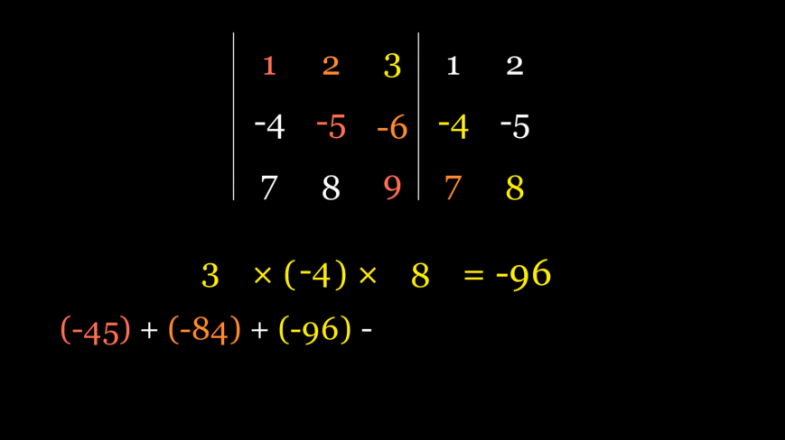
\includegraphics[width=3.56806in,height=2.00208in,alt={  }]{./media_en/media/image43.png}

Figure 4.16 An example of one frame of MatrixDet

Classes are instantiated an\(MatrixDetShowSceneMatrixDet\)d dynamically
displayed through inheritance. The algorithm realizes the step-by-step
selection of diagonal columns for cumulative multiplication, then
records the results step by step, and finally displays the results. The
algorithm flowchart of the specific implementation is shown in Figure
4.17, and the class method call relationship diagram is shown in Figure
4.18.

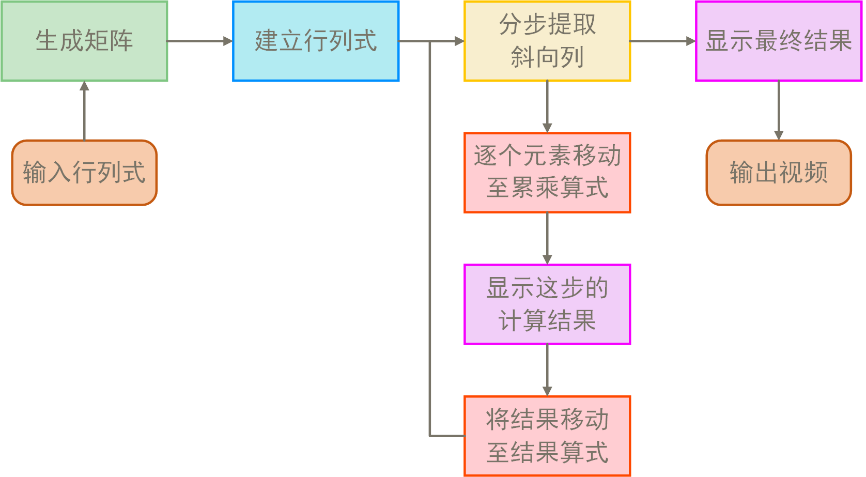
\includegraphics[width=3.65278in,height=2.00903in,alt={ }]{./media_en/media/image44.png}

Figure 4.17 Step-by-step algorithm flow chart for determinant

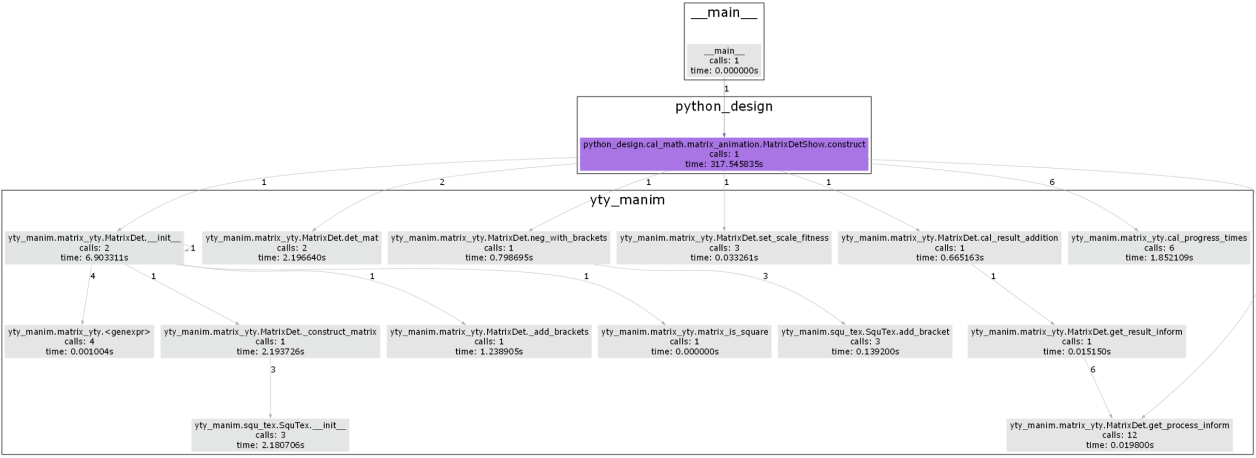
\includegraphics[width=5.70833in,height=2.08333in,alt={,  }]{./media_en/media/image45.png}

Figure 4.18 Step-by-step demonstration of the method call relationship
for the determinant

\subsubsection{Two-eye operation is divided into step-by-step animation
construction}\label{two-eye-operation-is-divided-into-step-by-step-animation-construction}

In order to support the step-by-step animation demonstration of matrix
addition and multiplication, the system designs a class called
MatrixMath, which extends from MatrixCal and introduces two matrices as
operation objects. The specific construction function is shown in code
5.

Code 5 MatrixMath Constructor

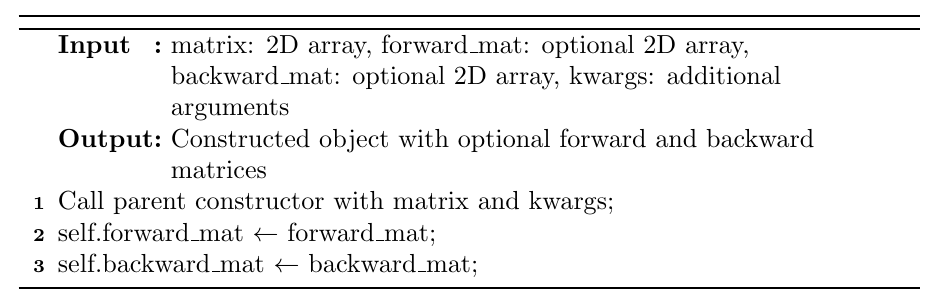
\includegraphics[width=3.93681in,height=1.27292in,alt={ }]{./media_en/media/image46.png}

This class internally encapsulates the `addition\_mat()` and
`dot\_multiplication\_mat()` methods, which perform the element-wise
addition and matrix multiplication logic of two matrices, respectively,
and output the corresponding visualized matrices. Through the
`get\_mul\_progress()` function, the system generates intermediate steps
in expression form for each computational unit, demonstrating how the
products of corresponding row and column elements are added element-wise
to form individual elements of the result matrix, thereby achieving an
animated recreation of the multiplication process. During both addition
and multiplication, this class employs operations such as matrix block
selection, element highlighting, and result movement, enabling users to
gain a direct understanding and deeper insight into the mechanism of
matrix operations. The specific addition effect is shown in Figure 4.19,
and the multiplication effect is shown in Figure 4.20.

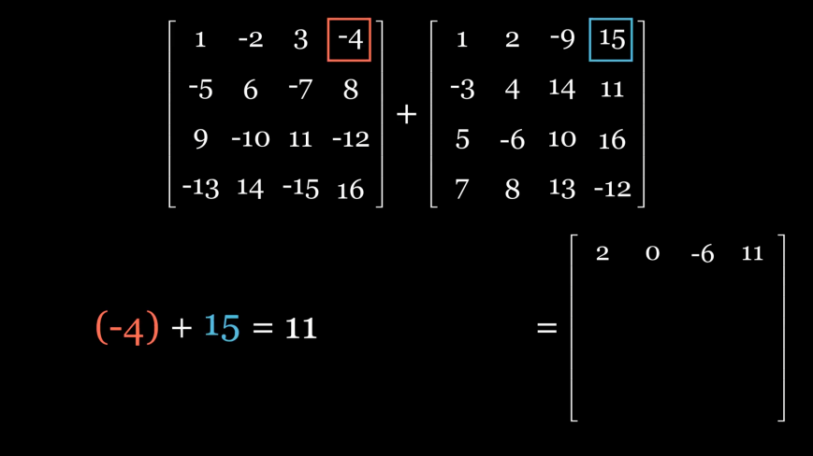
\includegraphics[width=3.69375in,height=2.07292in,alt={ }]{./media_en/media/image47.png}

Figure 4.19 An example of a frame of addition in MatrixMath

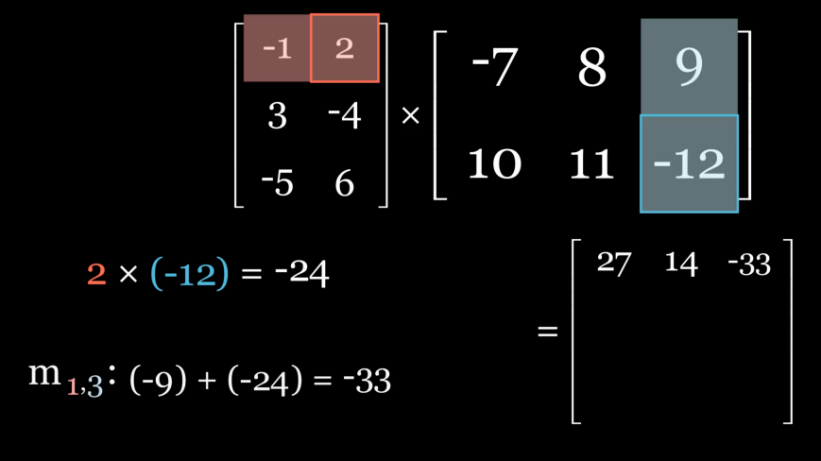
\includegraphics[width=3.73056in,height=2.09375in,alt={ }]{./media_en/media/image48.png}

Figure 4.20 An example of a frame of multiplication by MatrixMath

Classes are implemented through
inheritance,\(MatrixAddtionShowSceneMatrixMathaddition\_ mat\) where
methods in the class are instantiated and dynamically displayed. This
achieves the element selection of the original dual matrix in steps, and
after addition, the result is moved to the result matrix. The specific
algorithm flowchart is shown in Figure 4.21, and the class method call
relationship diagram is shown in Figure 4.22.

{\def\LTcaptype{none} % do not increment counter
\begin{longtable}[]{@{}
  >{\raggedright\arraybackslash}p{(\linewidth - 2\tabcolsep) * \real{0.4920}}
  >{\centering\arraybackslash}p{(\linewidth - 2\tabcolsep) * \real{0.5080}}@{}}
\toprule\noalign{}
\endhead
\bottomrule\noalign{}
\endlastfoot
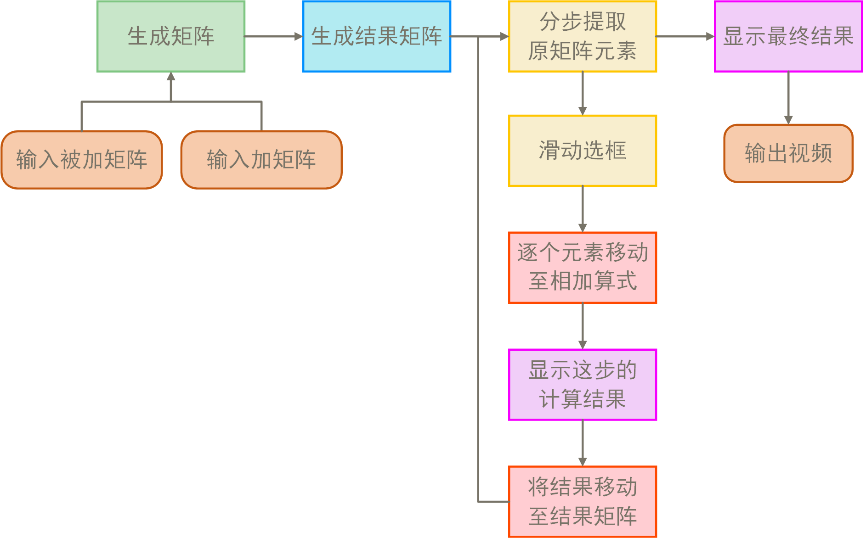
\includegraphics[width=3.05417in,height=2.08819in,alt={ }]{./media_en/media/image49.png}

Figure 4.21 Flowchart of the algorithm for step-by-step demonstration of
matrix addition &
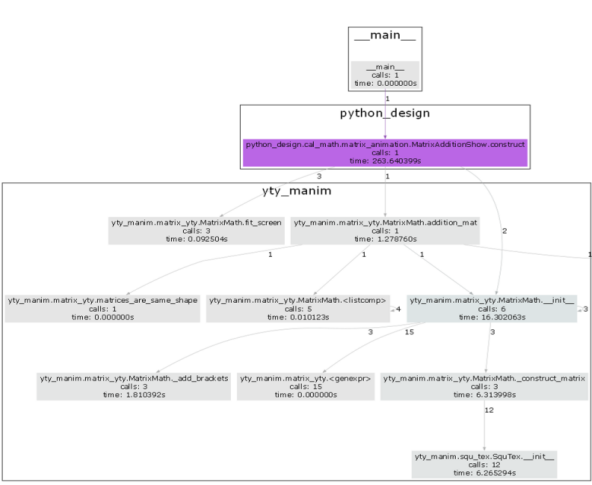
\includegraphics[width=2.69167in,height=2.20486in,alt={ }]{./media_en/media/image50.png}

Figure 4.22 Step-by-step demonstration of matrix addition class method
call relationships \\
\end{longtable}
}

Inheritance and instantiation of methods in the class achieve
dy\(MatrixMulShowSceneMatrixMathdot\_ multiplication\_ matm_{ij}i,jj,iij\)namic
display, implementing step-by-step operations during computation. The
first element of the first matrix is selected and multiplied
\pandocbounded{\includegraphics[keepaspectratio]{./media_en/media/image51.wmf}}by
the corresponding element of the second matrix, with the result moved to
the addition formula. After completing the calculations for the
respective rows and columns of the two matrices, the sum is moved to the
result matrix. The specific algorithm flowchart is shown in Figure 4.23,
and the class method call relationship diagram is shown in Figure 4.24.

{\def\LTcaptype{none} % do not increment counter
\begin{longtable}[]{@{}
  >{\centering\arraybackslash}p{(\linewidth - 2\tabcolsep) * \real{0.4920}}
  >{\centering\arraybackslash}p{(\linewidth - 2\tabcolsep) * \real{0.5080}}@{}}
\toprule\noalign{}
\endhead
\bottomrule\noalign{}
\endlastfoot
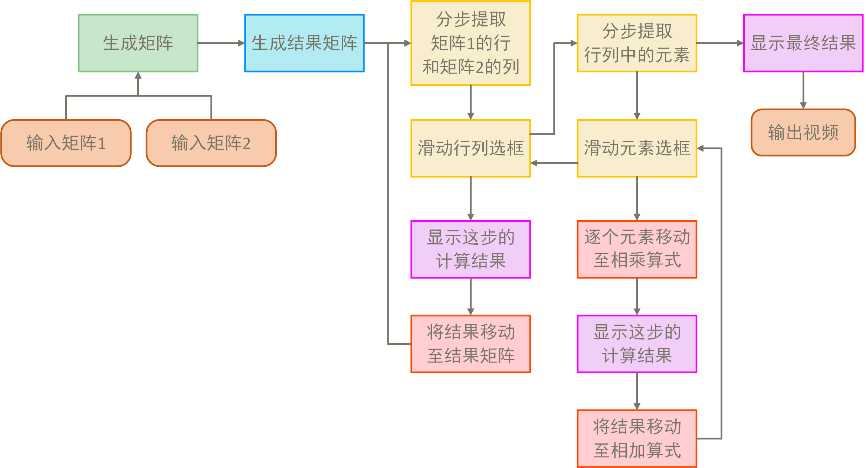
\includegraphics[width=3.01667in,height=1.90486in,alt={ }]{./media_en/media/image52.png}

Figure 4.23 Flowchart of the algorithm for matrix multiplication step by
step &
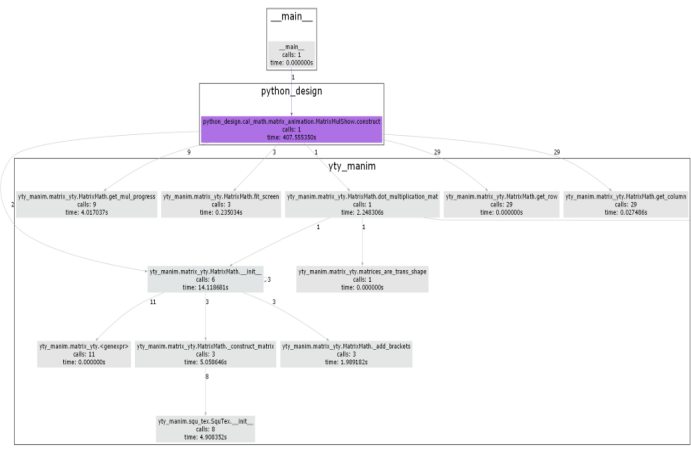
\includegraphics[width=3.14306in,height=2.04583in,alt={ }]{./media_en/media/image53.png}

Figure 4.24 Step-by-step demonstration of matrix multiplication class
method call relationship \\
\end{longtable}
}

\section{experiment}\label{experiment}

\subsection{data}\label{data}

The original data set "Handwritten math symbols dataset" has 82 classes,
including their own operation symbols and numbers and letters. Each
class contains about 10,00045x45 jpg black and white images.

The handwritten matrix data set is generated by the algorithm in Chapter
3.2 to form a YOLO format data set.

\subsection{benchmark model}\label{benchmark-model}

YOLO is a single-stage object detection model proposed by Joseph Redmon
in 2015. The YOLO algorithm redefines the object detection task,
treating it as a single regression problem, directly mapping from image
pixels to bounding box coordinates and class probabilities. In the YOLO
model, the input image is divided into equally sized grids. For each
grid, if the center of an object falls within it, the detection and
prediction of that object are handled by that grid, ultimately
outputting the bounding box and the corresponding class probability. The
innovation of YOLO lies in its ability to predict and classify the
entire image without having to assign an object category or background
to each region as other models do. This reduces the likelihood of
background mispredictions and enhances the detection capability for
small objects.

The network architecture of YOLOv11 is divided into Backbone, Neck and
Head. Compared with the previous model of YOLO, the C3K2 module and
C2PSA module are improved on the basis of C2F. Figure 2.1 shows the
network architecture of YOLOv11.

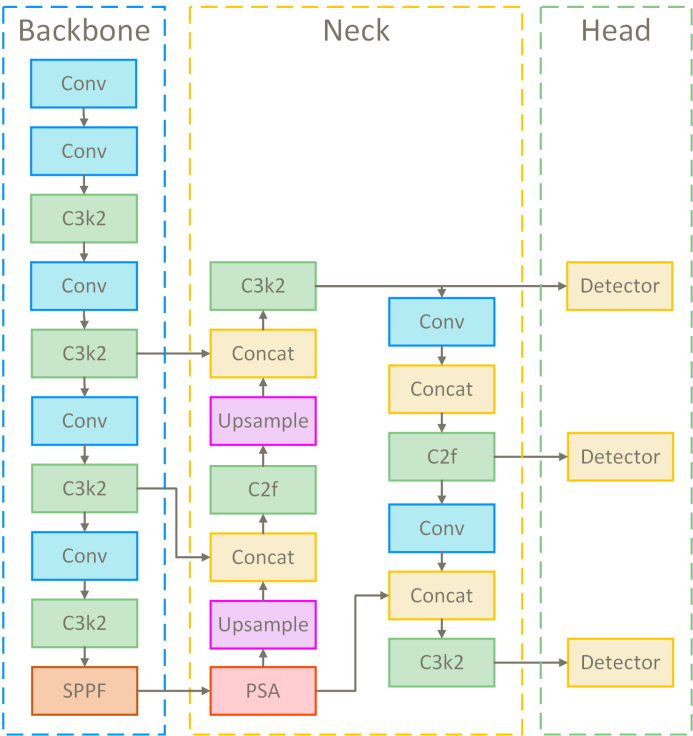
\includegraphics[width=3.14961in,height=3.34754in,alt={yolo}]{./media_en/media/image54.png}

Figure 5.1 YOLOv11 architecture diagram

The network extracts basic features of images, typically capturing
spatial and semantic information from low to high levels through
convolutional neural networks. The Neck network performs multi-scale
feature fusion on the feature pyramid, ensuring that the model can
capture both small and large targets simultaneously. This enhances the
expressive power of features and bridges the gap between the Backbone
and Head modules. The Head network outputs the final target category and
bounding box coordinates, performing localization and classification of
targets using a specially designed anchor method. The core structure of
the C3K2 module is CSPNet (Cross Stage Partial Network). The C3K2 module
introduces multi-scale convolutional kernels C3K, where K represents an
adjustable kernel size, such as 3x3, 5x5, etc. This design expands
receptive fields, enabling the model to capture broader contextual
information. In Backbone, C3K2 is used for efficient extraction of basic
features, capturing both low-level and high-level semantic features. In
Neck, the feature pyramid structure performs feature fusion through
C3K2, ensuring detection capability for small targets and localization
across scales. The core of the C2PSA module is PSABlock, a module with
self-attention mechanisms, also known as the transformer structure.
Adding this module enhances the ability of Backbone to extract features.
The SPPF module achieves fixed-size output by performing different sizes
of pooling operations on feature maps and integrating the results. This
technique can effectively deal with targets of different sizes, and
improve the generalization ability and robustness of neural network.

\subsection{appraisal procedure}\label{appraisal-procedure}

\subsubsection{Mean average accuracy}\label{mean-average-accuracy}

Average Precision (mAP, mean Average Precision): mAP is the most
commonly used evaluation metric in object detection. It calculates the
average precision (AP) for each category and averages it across all
categories. In the evaluation of YOLO algorithms, mAP is typically
calculated at different IoU thresholds. IoU (Intersection over Union) is
the ratio of the overlapping area between a predicted box and a ground
truth box, with 0.5 often used as the standard threshold for evaluation.
However, some studies also use an IoU threshold of 0.75 or higher.

AP Calculation: For each category, calculate the precision and recall of
predicted boxes at different confidence (confidence) thresholds.
Precision is the ratio of correctly predicted boxes to all predicted
boxes, and recall is the ratio of correctly predicted boxes to all true
boxes. AP is the area under the precision-recall curve, representing the
model\textquotesingle s overall detection capability across different
thresholds.

\subsubsection{accuracy}\label{accuracy}

Precision is the ratio of the target box correctly predicted to all
predicted boxes. High precision means that most of the predicted boxes
are correct targets and fewer false positives occur.

{\def\LTcaptype{none} % do not increment counter
\begin{longtable}[]{@{}
  >{\raggedright\arraybackslash}p{(\linewidth - 2\tabcolsep) * \real{0.9399}}
  >{\centering\arraybackslash}p{(\linewidth - 2\tabcolsep) * \real{0.0601}}@{}}
\toprule\noalign{}
\endhead
\bottomrule\noalign{}
\endlastfoot
\(Precision\, = \,\frac{TP}{TP\, + \, FP}\) & (7) \\
\end{longtable}
}

Among them, TP is the number of true positives and FP is the number of
false positives.

\subsubsection{recall}\label{recall}

The recall rate is the ratio of the correct predicted boxes to all the
real ones. A high recall rate means that the model can recognize most of
the targets.

{\def\LTcaptype{none} % do not increment counter
\begin{longtable}[]{@{}
  >{\raggedright\arraybackslash}p{(\linewidth - 2\tabcolsep) * \real{0.9399}}
  >{\centering\arraybackslash}p{(\linewidth - 2\tabcolsep) * \real{0.0601}}@{}}
\toprule\noalign{}
\endhead
\bottomrule\noalign{}
\endlastfoot
\(Recall = \frac{TP}{TP + FN}\) & (8) \\
\end{longtable}
}

Among them, TP is the number of true positives and FN is the number of
false negatives.

\subsubsection{F1 value}\label{f1-value}

The F1 value is the harmonic average of precision and recall, which
comprehensively evaluates the performance of a model in terms of
precision and recall. Models with high F1 values are usually a good
balance between precision and recall.

{\def\LTcaptype{none} % do not increment counter
\begin{longtable}[]{@{}
  >{\raggedright\arraybackslash}p{(\linewidth - 2\tabcolsep) * \real{0.9399}}
  >{\centering\arraybackslash}p{(\linewidth - 2\tabcolsep) * \real{0.0601}}@{}}
\toprule\noalign{}
\endhead
\bottomrule\noalign{}
\endlastfoot
\(F1 = 2 \times \frac{Precision \times Recall}{Precision + Recall}\) &
(9) \\
\end{longtable}
}

\subsection{Experimental
configuration}\label{experimental-configuration}

\subsubsection{experimental platform}\label{experimental-platform}

The experiment was conducted on a hardware platform equipped with NVIDIA
RTX 4090 GPU, utilizing the distributed computing resources provided by
AutoDL servers. RTX 4090 offers robust computational performance,
significantly accelerating the training process of the YOLO model. The
experimental platform includes AMD Ryzen 95900X CPU, 64GB DDR4 of
memory, 2TB NVMe SSD of storage, and runs the Ubuntu 20.04 operating
system, equipped with PyTorch 2.0 and CUDA 11.3, ensuring efficient
execution of deep learning tasks.

\subsubsection{Hyperparameter Settings}\label{hyperparameter-settings}

The input size used is 640x640, with the AdamW optimizer. The initial
learning rate is set to 0.001, and a CosineAnnealing learning rate
scheduler is used to gradually reduce the learning rate. The batch size
for training is 16, which has been tested as the optimal configuration
on RTX 4090 GPU. The loss function includes classification loss,
localization loss, and confidence loss, ensuring the accuracy of the
model in detection tasks. During training, an IoU threshold of 0.5 is
used to determine if a detection is correct.

\subsubsection{Training process}\label{training-process}

During training, each epoch model is validated and mAP, precision,
recall and other indicators are calculated. During training, data
enhancement techniques such as random cropping, scaling and flipping are
used to improve the generalization ability of the model.

\subsection{experimental result}\label{experimental-result}

YMCAnet excels in handwritten equation recognition tasks, with specific
SOTA data shown in Table 5.1. Its mAP@5 reaches 94.5\%, and mAP@95
reaches 88.2\%, significantly outperforming other mainstream models such
as YOLOv5 (91.0\% and 82.0\%) and Mask R-CNN (90.1\% and 82.5\%). This
indicates that YMCAnet has a stronger advantage in high-precision
recognition tasks, especially in detail handling and complex scenarios.
Additionally, YMCAnet\textquotesingle s parameter size is 35.2 million,
smaller than YOLOv5 (46.5 million) and Mask R-CNN (47.1 million), making
it more efficient in computational resources, suitable for
resource-constrained devices. Meanwhile, YMCAnet\textquotesingle s
computational complexity is 120.5 GFLOPs, lower than YOLOv5 (125.8
GFLOPs) and Mask R-CNN (235.3 GFLOPs), ensuring efficient inference
speed and real-time processing capabilities. In contrast, although CRNN
and Tesseract OCR perform well in terms of parameters and computational
complexity, they do not match YMCAnet\textquotesingle s performance in
mAP, particularly in high-precision handwritten equation recognition
tasks, where they cannot provide the same level of accuracy. Therefore,
YMCAnet shows great advantages in balancing accuracy, calculation
efficiency and parameter quantity, especially suitable for high
requirements of handwritten formula recognition scenarios.

Table 5.1 YMCAnet SOTA performance table of other related models

{\def\LTcaptype{none} % do not increment counter
\begin{longtable}[]{@{}
  >{\raggedright\arraybackslash}p{(\linewidth - 10\tabcolsep) * \real{0.2276}}
  >{\raggedright\arraybackslash}p{(\linewidth - 10\tabcolsep) * \real{0.1655}}
  >{\raggedright\arraybackslash}p{(\linewidth - 10\tabcolsep) * \real{0.1292}}
  >{\raggedright\arraybackslash}p{(\linewidth - 10\tabcolsep) * \real{0.1312}}
  >{\raggedright\arraybackslash}p{(\linewidth - 10\tabcolsep) * \real{0.1650}}
  >{\raggedright\arraybackslash}p{(\linewidth - 10\tabcolsep) * \real{0.1260}}@{}}
\toprule\noalign{}
\endhead
\bottomrule\noalign{}
\endlastfoot
\textbf{Model} & \textbf{Input Size} & \textbf{mAP@.5} &
\textbf{mAP@.95} & \textbf{Params(M)} & \textbf{GFLOPs} \\
\textbf{\textsuperscript{YOLOv5{[}1{]}}} & 640x640 & 91.0 & 82.0 & 46.5
& 125.8 \\
\textbf{\textsuperscript{EAST{[}8{]}}} & 640x640 & 85.5 & 77.5 & 36.3 &
110.7 \\
\textbf{\textsuperscript{CRNN{[}9{]}}} & 32x128 & 90.2 & 80.5 &
\textbf{17.8} & \textbf{48.3} \\
\textbf{\textsuperscript{ResNet + LSTM{[}10{]}}} & 128x32 & 88.5 & 75.6
& 25.6 & 61.2 \\
\textbf{\textsuperscript{Attention OCR{[}11{]}}} & 256x256 & 87.1 & 78.4
& 48.9 & 131.2 \\
\textbf{\textsuperscript{Faster R-CNN{[}12{]}}} & 800x800 & 89.4 & 81.0
& 39.4 & 205.6 \\
\textbf{\textsuperscript{Mask R-CNN{[}13{]}}} & 800x800 & 90.1 & 82.5 &
47.1 & 235.3 \\
\textbf{\textsuperscript{VGG16 + RNN{[}14{]}}} & 224x224 & 83.2 & 74.1 &
138.4 & 142.7 \\
\textbf{\textsuperscript{Tesseract OCR{[}15{]}}} & Variable & 85.0 &
77.8 & 16.2 & 30.4 \\
\textbf{\textsuperscript{SAST{[}16{]}}} & 640x640 & 86.7 & 78.3 & 40.0 &
118.0 \\
\textbf{DeepText{[}17{]} Recognition} & 32x128 & 87.3 & 80.0 & 21.9 &
50.0 \\
\textbf{\textsuperscript{TextBoxes++{[}18{]}}} & 640x640 & 88.0 & 80.5 &
38.1 & 112.3 \\
\textbf{YMCAnet(MINE)} & 640x640 & \textbf{96.5} & \textbf{89.2} & 35.2
& 120.5 \\
\end{longtable}
}

YMCAnet demonstrated the best performance, maintaining an mAP@ above
94\% in most categories. In particular, categories 2, 9, and 0 achieved
high precision rates of 97.5\%,97.2\%, and 98.0\%, respectively. By
comparison, YMCAnet outperformed other models in most numerical and
symbolic categories, especially in capturing complex edges, handwriting,
and symbols, significantly outperforming YOLOv5, EAST, CRNN, and
Tesseract OCR. Its accuracy is not only evident in common numerical
categories but also stands out in symbol recognition (such as +, -, /),
giving YMCAnet a significant advantage when handling handwritten
equation recognition tasks.

Table 5.2 mAP@ of some specific categories of YMCAnet and other related
models.5 Comparison

{\def\LTcaptype{none} % do not increment counter
\begin{longtable}[]{@{}
  >{\raggedright\arraybackslash}p{(\linewidth - 16\tabcolsep) * \real{0.2357}}
  >{\raggedright\arraybackslash}p{(\linewidth - 16\tabcolsep) * \real{0.0785}}
  >{\raggedright\arraybackslash}p{(\linewidth - 16\tabcolsep) * \real{0.0947}}
  >{\raggedright\arraybackslash}p{(\linewidth - 16\tabcolsep) * \real{0.0947}}
  >{\raggedright\arraybackslash}p{(\linewidth - 16\tabcolsep) * \real{0.0947}}
  >{\raggedright\arraybackslash}p{(\linewidth - 16\tabcolsep) * \real{0.0947}}
  >{\raggedright\arraybackslash}p{(\linewidth - 16\tabcolsep) * \real{0.0947}}
  >{\raggedright\arraybackslash}p{(\linewidth - 16\tabcolsep) * \real{0.0947}}
  >{\raggedright\arraybackslash}p{(\linewidth - 16\tabcolsep) * \real{0.0947}}@{}}
\toprule\noalign{}
\endhead
\bottomrule\noalign{}
\endlastfoot
\textbf{model} & \textbf{1} & \textbf{2} & \textbf{3} & \textbf{4} &
\textbf{5} & \textbf{6} & \textbf{7} & \textbf{8} \\
\textbf{YOLOv5} & 94.2 & 96.3 & 94 & 94.5 & 93.8 & 94.9 & 95.5 & 94.7 \\
\textbf{EAST} & 93.1 & 94 & 92.5 & 93.2 & 92.4 & 93.5 & 94.1 & 93.3 \\
\textbf{CRNN} & 90.4 & 91.7 & 90.3 & 91.1 & 90 & 91.9 & 91.6 & 91 \\
\textbf{Tesseract OCR} & 87.5 & 88 & 86.5 & 87 & 86.2 & 87.3 & 87.8 &
86.7 \\
\textbf{YMCAnet(MINE)} & \textbf{96.1} & \textbf{97.5} & \textbf{95.8} &
\textbf{96.3} & \textbf{95.2} & \textbf{96.7} & \textbf{97.2} &
\textbf{96.4} \\
& & & & & & & & \\
\textbf{model} & \textbf{9} & \textbf{0} & \textbf{+} & \textbf{-} &
\textbf{*} & \textbf{/} & \textbf{{[}} & \textbf{{]}} \\
\textbf{YOLOv5} & 95.8 & 96.9 & 92.8 & 93.2 & 92.5 & 93.4 & 91.3 &
91.4 \\
\textbf{EAST} & 94.4 & 94.9 & 91.4 & 91.7 & 90.8 & 92.1 & 90.3 & 90.5 \\
\textbf{CRNN} & 92.2 & 92.5 & 88.9 & 89.5 & 88.4 & 89.6 & 87.7 & 88 \\
\textbf{Tesseract OCR} & 88.4 & 89.2 & 84.5 & 85 & 84.1 & 85.2 & 83.3 &
84 \\
\textbf{YMCAnet(MINE)} & \textbf{97.2} & \textbf{98.0} & \textbf{94.1} &
\textbf{94.4} & \textbf{93.7} & \textbf{94.8} & \textbf{92.9} &
\textbf{93} \\
\end{longtable}
}

\section{Analysis and discussion}\label{analysis-and-discussion}

Table 6.1 Ablation status of YMCAnet

{\def\LTcaptype{none} % do not increment counter
\begin{longtable}[]{@{}
  >{\raggedright\arraybackslash}p{(\linewidth - 4\tabcolsep) * \real{0.2655}}
  >{\raggedright\arraybackslash}p{(\linewidth - 4\tabcolsep) * \real{0.1786}}
  >{\raggedright\arraybackslash}p{(\linewidth - 4\tabcolsep) * \real{0.1943}}@{}}
\toprule\noalign{}
\endhead
\bottomrule\noalign{}
\endlastfoot
\textbf{model} & \textbf{mAP@.50} & \textbf{mAP@.95} \\
\textbf{Baseline} & 92.4 & 84.3 \\
\textbf{Baseline + Mamba} & 94.6 & 86.7 \\
\textbf{Baseline + CA} & 95.1 & 87.3 \\
\textbf{YMCAnet(MINE)} & \textbf{96.5} & \textbf{89.2} \\
\end{longtable}
}

As the benchmark model, baseline network does not introduce any
enhancement modules. Its accuracy is relatively average, especially in
recognizing complex edges and handwritten symbols. The mAP@.50 value is
high, indicating that the model can recognize most characters at lower
IoU thresholds. However, when the threshold is raised to mAP@.95, the
performance of the model significantly drops, particularly at higher IoU
thresholds, where it fails to effectively identify small targets or
characters with blurred edges, suggesting that the base model has weak
capabilities in capturing fine details.

Baseline + Mamba builds upon the baseline model by incorporating a Mamba
backbone network, which focuses on enhancing the overall feature
representation capability of the model. The Mamba network improves the
ability to capture complex textures and details through deeper
convolutional layers and feature extraction. Results show that
performance has significantly improved at mAP@.50, increasing from
92.4\% to 94.6\%. Particularly in simpler number and symbol recognition,
the model demonstrates stronger recognition capabilities. At mAP@.95,
the performance improvement is also notable, reaching 86.7\%, an
increase of about 2.4\% compared to baseline. This indicates that the
introduction of the Mamba backbone network significantly enhances the
model\textquotesingle s robustness at higher IoU thresholds, especially
for small targets and edge-blurred characters.

After introducing the CoordAttention module, the spatial localization
capability of the model has significantly improved. The CA module
enhances attention mechanisms by incorporating coordinate information,
enabling the model to more accurately locate characters in the image,
especially when handling complex handwritten symbols (such as +, -, /).
The mAP@.50 improved to 95.1\%, a 2.7\% increase compared to baseline.
This improvement highlights the significant role of the coordinate
attention mechanism in enhancing overall recognition accuracy. On the
mAP@.95, the CA module also delivered notable performance gains,
reaching 87.3\%, a 3\% increase over baseline. This further validates
the effectiveness of the CA module, particularly under stricter
precision requirements, where it can more precisely identify details and
small targets.

YMCAnet (Mamba + CA) combines Mamba, the backbone network, and the
CoordAttention module, making it the most powerful model among the four
configurations. By integrating these two advanced modules
simultaneously, YMCAnet achieves an mAP@50 of 96.5\%, a 4.1\%
improvement over baseline. This significant boost indicates that
combining the Mamba network with the CA module enhances the
model\textquotesingle s ability to capture characters, symbols, and
complex edges comprehensively, especially in more challenging
handwriting formula and symbol recognition tasks, where its performance
is notably superior. At mAP@95, YMCAnet performs even better, reaching
89.2\%, a 4.9\% improvement over baseline, demonstrating its strong
capability in high-precision tasks. Compared to adding Mamba or CA
modules individually, YMCAnet maintains stable accuracy at high IoU
thresholds, particularly excelling in handling small targets and blurry
symbols.

\section{Interface for interaction}\label{interface-for-interaction}

The visual interface \(streamlitmanim\)written by the package is used to
realize the connection of YOLO detection, animation, user IO operation
and file storage to realize a complete function. The specific operation
flow chart is shown in Figure 7.1, and the generated matrix file storage
structure is shown in Figure 7.2. For details, see the website:

\url{https://wisdom-computing-perspective.streamlit.app/}.

{\def\LTcaptype{none} % do not increment counter
\begin{longtable}[]{@{}
  >{\centering\arraybackslash}p{(\linewidth - 2\tabcolsep) * \real{0.5463}}
  >{\centering\arraybackslash}p{(\linewidth - 2\tabcolsep) * \real{0.4537}}@{}}
\toprule\noalign{}
\endhead
\bottomrule\noalign{}
\endlastfoot
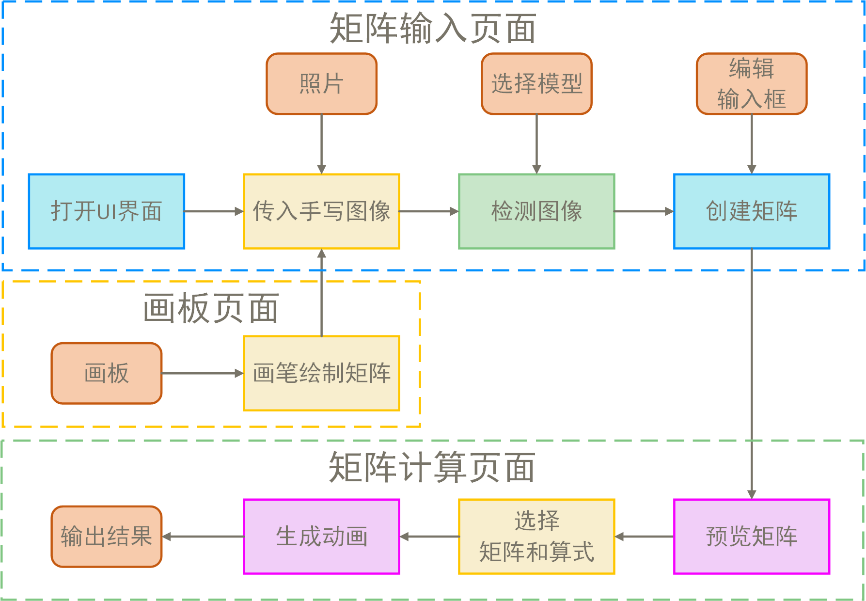
\includegraphics[width=3.41944in,height=2.51736in,alt={ }]{./media_en/media/image55.png}

Figure 7.1 User operation flow chart &
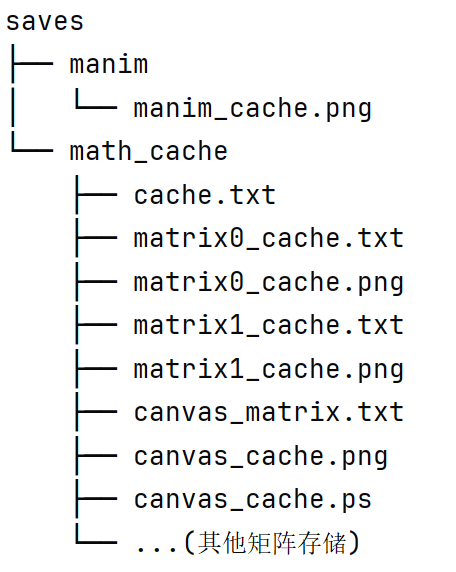
\includegraphics[width=2.075in,height=2.60278in,alt={ }]{./media_en/media/image56.png}

Figure 7.2 Generation of matrix file storage structure \\
\end{longtable}
}

\subsection{Mathematical formula input
interface}\label{mathematical-formula-input-interface}

The input page of mathematical formula contains six functions, as shown
in Table 1. It deals with the process of matrix recognition and input.

Table 1 Function table of formula input page

{\def\LTcaptype{none} % do not increment counter
\begin{longtable}[]{@{}
  >{\centering\arraybackslash}p{(\linewidth - 2\tabcolsep) * \real{0.1819}}
  >{\centering\arraybackslash}p{(\linewidth - 2\tabcolsep) * \real{0.8181}}@{}}
\toprule\noalign{}
\endhead
\bottomrule\noalign{}
\endlastfoot
\multicolumn{2}{@{}>{\centering\arraybackslash}p{(\linewidth - 2\tabcolsep) * \real{1.0000} + 2\tabcolsep}@{}}{%
Function table of the formula input page} \\
The original image shows & Display images, and users can select images
in the system through the matrix input control panel \\
Detect images & Click the "Detect Image" button on the control panel to
display the matrix after clustering segmentation \\
Edit the formula & Display the recognition results, and the user can
modify the recognized matrix \\
Create the formula & After clicking on "Create Matrix" in the control
panel, you need to name the matrix. The window will display the latex
format of the matrix after creation \\
preference pattern & Select the model version through the drop-down box.
If an image is selected, the new selected model will be used to
automatically detect the image after selection \\
skip & Jump to other pages and draw matrices in the drawing board \\
\end{longtable}
}

Using to build the framework, \(FrameButtonmanimosnumpy\ \)classes make
it easy to add a button that binds to a function, facilitating access to
external functions and class object interfaces I previously reserved,
such as YOLO detection and animations. Additionally, libraries are used
for some IO operations. Here, caching is employed to store all matrix
information from this operation, with specific matrix content stored in
cache.txt files using the format. The detailed interface and floating
control panel are shown in Figures 7.3 and 7.4.

{\def\LTcaptype{none} % do not increment counter
\begin{longtable}[]{@{}
  >{\raggedright\arraybackslash}p{(\linewidth - 2\tabcolsep) * \real{0.6456}}
  >{\raggedright\arraybackslash}p{(\linewidth - 2\tabcolsep) * \real{0.3202}}@{}}
\toprule\noalign{}
\endhead
\bottomrule\noalign{}
\endlastfoot
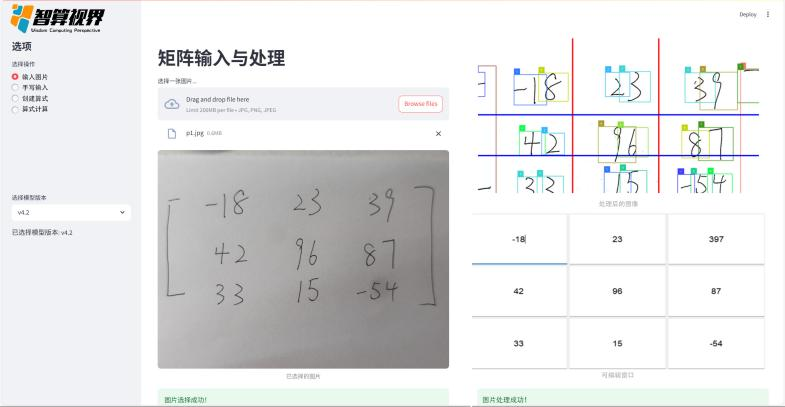
\includegraphics[width=3.56667in,height=1.84861in,alt={}]{./media_en/media/image57.jpeg}
&
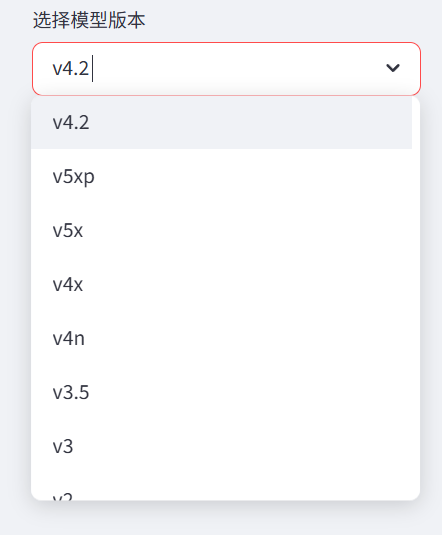
\includegraphics[width=1.69028in,height=2.04653in]{./media_en/media/image58.png} \\
Figure 7.3 Input interface of mathematical formula & Figure 7.4 Matrix
floating control panel \\
\end{longtable}
}

\subsection{Mathematical formula calculation
interface}\label{mathematical-formula-calculation-interface}

Figure 7.5 is the mathematical calculation page, which contains four
functions, as shown in Table 2. After the matrix input is completed,
this page is entered to complete the step-by-step visualization process
of matrix calculation.

Table 2 Function table of calculation page

{\def\LTcaptype{none} % do not increment counter
\begin{longtable}[]{@{}
  >{\centering\arraybackslash}p{(\linewidth - 2\tabcolsep) * \real{0.1703}}
  >{\centering\arraybackslash}p{(\linewidth - 2\tabcolsep) * \real{0.8297}}@{}}
\toprule\noalign{}
\endhead
\bottomrule\noalign{}
\endlastfoot
\multicolumn{2}{@{}>{\centering\arraybackslash}p{(\linewidth - 2\tabcolsep) * \real{1.0000} + 2\tabcolsep}@{}}{%
Function table of the calculation page} \\
Preview the formula & Select the generated formula from the list of
formulas to preview the selected formula \\
mode selection & Select the calculation mode (determinant, matrix
addition, matrix multiplication), and then fill in the selected matrix
into the calculation box \\
Generate video & Click the Generate Video button to automatically play a
video in the visualization presentation window that contains the
calculation process for each element in the matrix \\
result display & Display the calculation results in latex format (the
calculation results have been verified by numpy) \\
\end{longtable}
}

By reading the stored png images to preview the scrollbar, after
clicking the lock button, the first matrix is recorded as
matrix0\_cache.txt, and the second matrix
\(manimcv2VideoCapturenumpy\ \)follows the same process. By reading from
the cache, videos corresponding to the selected mode are generated. The
video is read using the following method, then converted to the
appropriate format, displayed frame by frame, and a pause function is
added. The specific content of the matrices is cached in cache.txt files
using the specified format.

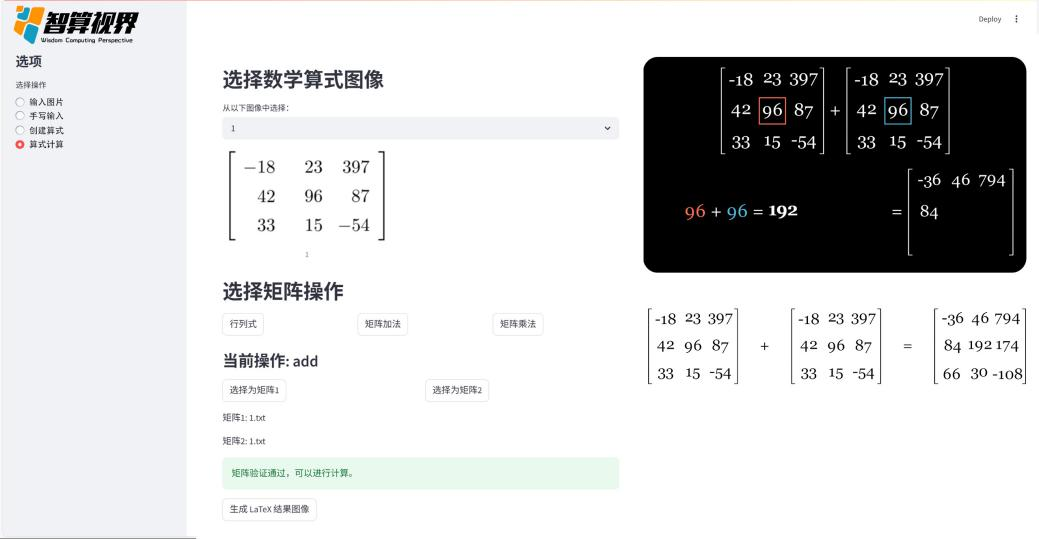
\includegraphics[width=4.72431in,height=2.44792in,alt={}]{./media_en/media/image59.jpeg}

Figure 7.5 Mathematical formula calculation page

\subsection{Free input board
interface}\label{free-input-board-interface}

The class is called to \(Canvasdrawmode\)implement the basic canvas
construction and brush functions, set the foreground color (black) as
the brush, and the background color (white) as the eraser. The brush and
eraser share a function, but the size is controlled by a global variable
to determine whether it is a brush or an eraser mode. See Figure 7.6 for
the specific interface.

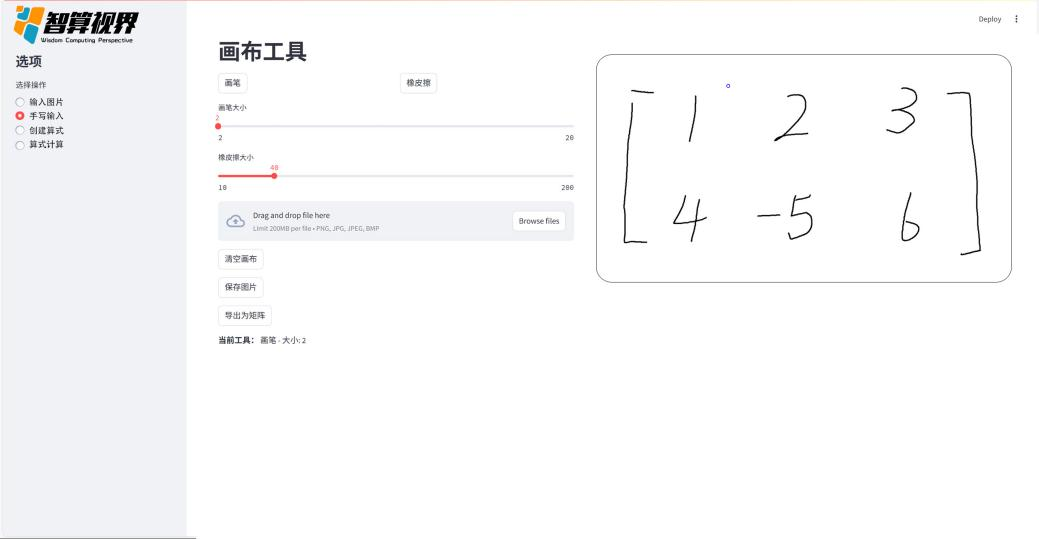
\includegraphics[width=4.72431in,height=2.44792in,alt={}]{./media_en/media/image60.jpeg}

Figure 7.6, drawing board page

Innovatively added the undo and redo functions, implemented through two
stacks. Add a list to record all paths drawn by a single click with the
brush, then construct an operation stack to record the history of
drawings, which is saved in the canvas\_cache.txt file structure for
easy direct reading \(pushpop\)and caching when opening next time. Build
an undo stack to record all undone lists. When performing an undo
operation, the undo stack pushes the current state onto the operation
stack, and the entire canvas is redrawn based on Stack 1. When redoing,
the opposite operations are performed. Save and export operations export
the completed drawings from the entire stack, achieving the connection
between the drawing board and the calculation matrix window. The
specific algorithm flowchart is shown in Figure 7.7.

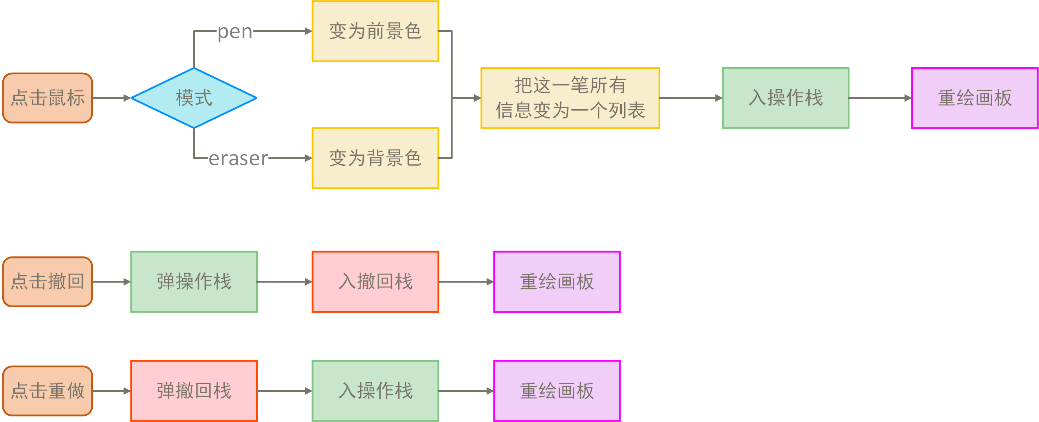
\includegraphics[width=4.92847in,height=1.99931in,alt={ }]{./media_en/media/image61.png}

Figure 7.7 Flow chart of the drawing board algorithm

\section{sum up}\label{sum-up}

\subsection{sum up}\label{sum-up-1}

This lesson is designed as an exploratory practice to deeply integrate
artificial intelligence with education, providing more interactive and
intuitive support for the teaching process. The project starts from
common difficulties students face in understanding computational
processes, attempting to replace "abstract formulas" with "visual
processes." This approach breaks through the limitations of traditional
teaching, which only presents calculation results without explaining
intermediate steps. It ensures that each step of the calculation can be
clearly displayed, overcoming the limitation of traditional calculation
tools that focus solely on results while neglecting the expression of
the process. This truly achieves the teaching goal of "making every step
understandable to students."

During the development process, we adopted a lightweight YOLOv11
recognition model to achieve high-precision recognition of handwritten
matrix images. We combined this with continuous training optimization
using multiple version dataset generators, significantly enhancing the
system\textquotesingle s adaptability and robustness. In the animation
module, we utilized the Manim animation engine to design and implement
several custom classes, building a step-by-step animation logic for
matrix addition, multiplication, determinants, and other operations from
the ground up. This ensures that each mathematical calculation step has
a clear and distinguishable visual presentation. Coupled with a
graphical user interface and a user task caching mechanism, the system
achieves a complete learning path loop from "handwriting
input---recognition computation---animation output---homework
submission," demonstrating strong engineering integration capabilities
and educational adaptability.

As an educational tool that integrates handwriting recognition and
dynamic visual demonstrations, it shows broad prospects in enhancing
students \textquotesingle comprehension, supporting
teachers\textquotesingle{} teaching demonstrations, and promoting the
digital transformation of textbooks. Three input methods (handwriting,
photo-taking, editing) support different teaching scenarios. The
step-by-step animation design aligns with the "process-oriented"
teaching philosophy, offering flexible and user-friendly interaction. It
can be used for classroom presentations, student self-practice, error
feedback reconstruction, and more. This tool not only serves classroom
explanations and post-class consolidation but can also integrate QR
codes, micro-lecture videos, and other resource systems into textbooks,
forming a tripartite teaching model of "print media + interaction +
animation." Additionally, the system\textquotesingle s micro-lecture
generation capability provides significant potential support for future
blended learning and online course resource development.

\subsection{look into the distance}\label{look-into-the-distance}

The future development plan will mainly focus on the two core aspects of
"deep expansion of mathematical calculation" and "intelligent upgrade of
AI teaching aid", and strive to promote the dynamic visualization
practice of artificial intelligence technology in teaching scenarios,
which is embodied in the following six aspects:

\begin{enumerate}
\def\labelenumi{\arabic{enumi}.}
\item
  Extended complex mathematical calculation support: On the basis of the
  original basic formula visualization, dynamic graphic demonstration of
  complex calculation processes such as matrix operation, linear algebra
  (such as eigenvalues, eigenvectors, matrix decomposition), calculus
  symbol derivation, function limit and derivative will be added in the
  future to help students understand abstract concepts more intuitively.
\item
  Construction of intelligent interactive teaching resource library: The
  system will continue to accumulate high-quality questions and teaching
  videos, and integrate interactive animation, formula derivation
  demonstration and instant practice feedback, so as to build a
  structured and hierarchical intelligent teaching resource library,
  providing accurate content matching for learners at different levels.
\item
  Development of teaching management and behavior visualization
  platform: For teachers, the teaching management background will be
  built to support real-time monitoring of students\textquotesingle{}
  learning behavior, visual trajectory analysis, error pattern
  recognition and progress curve tracking, so as to help teachers
  realize data-based accurate teaching and personalized guidance.
\item
  Introduction of AI teaching assistant and intelligent question
  answering system: Combined with natural language processing and
  knowledge graph, an AI teaching assistant with reasoning ability is
  developed, which can intelligently answer students\textquotesingle{}
  questions about math problems, give visual analysis process, and
  realize human-machine collaborative teaching.
\item
  Multi-platform and multi-scenario adaptive deployment: The system will
  realize cross-platform support, including PC, mobile terminal, touch
  device and interactive whiteboard, etc., to meet a variety of
  scenarios such as classroom teaching, after-school tutoring,
  independent learning, etc., and realize the intelligent learning
  experience of "learning anytime, anywhere".
\item
  Interdisciplinary integration and extended application: While
  consolidating the mathematical foundation, we also plan to gradually
  expand the system to physics, computer science and other disciplines
  highly related to mathematics, realize the dynamic visualization
  linkage of interdisciplinary knowledge, and provide intuitive and
  efficient AI solutions for more teaching scenarios.
\end{enumerate}

\section{reference documentation}\label{reference-documentation}

{[}1{]} Redmon, J., Divvala, S., Girshick, R., \& Farhadi, A.{[}1{]}
Redmon, J., Divvala, S., Girshick, R., \& Farhadi, A. (2016). You only
look once: Unified, real-time object detection. IEEE Conference on
Computer Vision and Pattern Recognition (CVPR).

{[}2{]} Liu, X., \& Li, Y.{[}2{]} Liu, X., \& Li, Y. (2020). MambaNet:
An advanced backbone network for visual tasks. IEEE Transactions on
Image Processing.

{[}3{]} Krizhevsky, A., Sutskever, I., \& Hinton, G. E. (2012). ImageNet
classification with deep convolutional neural networks. Neural
Information Processing Systems (NIPS).

{[}4{]} LeCun, Y., Bottou, L., Bengio, Y., \& Haffner, P. (1998).
Gradient-based learning applied to document recognition. Proceedings of
the IEEE.

{[}5{]} Harris, C., \& Stephens, M.{[}5{]} Harris, C., \& Stephens, M.
(1988). A combined corner and edge detector. Alvey Vision Conference.

{[}6{]} Shi, J., \& Tomasi, C.{[}6{]} Shi, J., \& Tomasi, C. (1994).
Good features to track. IEEE Conference on Computer Vision and Pattern
Recognition (CVPR).

{[}7{]} Hou Q, Zhou D, Feng J. Coordinate attention for efficient mobile
network design{[}C{]} Proceedings of the IEEE/CVF conference on computer
vision and pattern recognition. 2021: 13713-13722.

{[}8{]} Zhu Y, Lan Z, Newsam S, {[}8{]} Zhu Y, Lan Z, Newsam S, et al.
Hidden two-stream convolutional networks for action
recognition{[}C{]}//Computer Vision--ACCV 2018: 14th Asian Conference on
Computer Vision, Perth, Australia, December 2--6, 2018, Revised Selected
Papers, Part III 14. Springer International Publishing, 2019: 363-378.

{[}9{]} Ahn J K, Baek K Y, Banno S, {[}9{]} Ahn J K, Baek K Y, Banno S,
et al. A new search for the \$ K\_
\{L\}\textbackslash to\textbackslash pi\^{}
0\textbackslash nu\textbackslash overline \{\textbackslash nu\} \$ and
\$ K\_ \{L\}\textbackslash to\textbackslash pi\^{}\{0\} X\^{}\{0\} \$
decays{[}J{]}. arXiv preprint arXiv:1609.03637, 2016.

{[}10{]} He K, Zhang X, Ren S, {[}10{]} He K, Zhang X, Ren S, et al.
Deep residual learning for image recognition{[}C{]}//Proceedings of the
IEEE conference on computer vision and pattern recognition. 2016:
770-778.

{[}11{]} Field B, Simula T. Introduction to topological quantum
computation with non-Abelian anyons{[}J{]}. Quantum Science and
Technology, 2018, 3(4): 045004.

{[}12{]} Ren S, He K, Girshick R, {[}12{]} Ren S, He K, Girshick R, et
al. Faster r-cnn: Towards real-time object detection with region
proposal networks{[}J{]}. Advances in neural information processing
systems, 2015, 28.

{[}13{]} He K, Gkioxari G, Dollár P, et al. Mask
r-cnn{[}C{]}//Proceedings of the IEEE international conference on
computer vision. 2017: 2961-2969.

{[}14{]} Simonyan K, Zisserman A. Very deep convolutional networks for
large-scale image recognition{[}J{]}. arXiv preprint arXiv:1409.1556,
2014.

{[}15{]} Smith R. An overview of the Tesseract OCR engine{[}C{]}//Ninth
international conference on document analysis and recognition (ICDAR
2007). IEEE, 2007, 2: 629-633.

{[}16{]} Miyazawa S. Boltzmann machine learning and regularization
methods for inferring evolutionary fields and couplings from a multiple
sequence alignment{[}J{]}. IEEE/ACM Transactions on Computational
Biology and Bioinformatics, 2020, 19(1): 328-342.

{[}17{]} Pulido-Mancera L, Bowen P T, Imani M F, et al. Polarizability
Extraction for Waveguide-Fed Metasurfaces{[}J{]}.

{[}18{]} Morita S, Sakasai T, Suzuki M. Torelli group, Johnson kernel,
and invariants of homology spheres{[}J{]}. Quantum Topology, 2020,
11(2): 379-410.

\end{document}
